%--------------------------------------------------------------------%
%
% Berkas utama templat LaTeX.
%
% author Petra Barus, Peb Ruswono Aryan, Faris Rizki Ekananda
%
%--------------------------------------------------------------------%
%
% Berkas ini berisi struktur utama dokumen LaTeX yang akan dibuat.
%
%--------------------------------------------------------------------%

\documentclass[bahasa, 12pt, a4paper, onecolumn, oneside, final]{report}

%-------------------------------------------------------------------%
%
% Konfigurasi dokumen LaTeX untuk laporan tesis IF ITB
%
% @author Petra Novandi
%
%-------------------------------------------------------------------%
%
% Berkas asli berasal dari Steven Lolong
%
%-------------------------------------------------------------------%

% Ukuran kertas
\special{papersize=210mm,297mm}

% Setting margin
\usepackage[top=2cm,bottom=2cm,left=4cm,right=3cm]{geometry}

% Math package
\usepackage{mathptmx}

% 4th Sectioning
\usepackage{titlesec}
\newcommand{\subsubsubsection}[1]{\paragraph{#1}\mbox{}\\}

\titleformat{\subsubsubsection}
{\normalfont\normalsize\bfseries}{\theparagraph}{1em}{}
\titlespacing*{\subsubsubsection}
{0pt}{3.25ex plus 1ex minus .2ex}{1.5ex plus .2ex}

% Judul bahasa Indonesia
\usepackage[bahasa]{babel}

% Format citation
\usepackage[utf8]{inputenc}
\usepackage[style=apa,backend=biber]{biblatex}
\usepackage{longtable}
\usepackage{graphicx}
\usepackage{subfig}
\usepackage{titling}
\usepackage{booktabs}
\usepackage{tabularx}
\usepackage{blindtext}
\usepackage{sectsty}
\usepackage{chngcntr}
\usepackage{etoolbox}
\usepackage{array}
\usepackage[hidelinks]{hyperref}       % Package untuk link di daftar isi. Ubah jadi \usepackage[hidelinks]{hyperref} apabila ingin menghilangkan kotak merah disekitar link
\usepackage{titlesec}       % Package Format judul
\usepackage{titletoc}       % Package Format judul di toc
\usepackage{tocbibind}      % Package untuk masukkan toc, lot, lof ke Daftar Isi
\usepackage{scrwfile}       % Package untuk membuat Daftar Lampiran dari toc
\usepackage{parskip}
\usepackage{afterpage}
\usepackage{relsize}
\usepackage{xcolor, colortbl}
\usepackage{setspace}
\usepackage{listings}

\graphicspath{{resources/}}   % letak direktori penyimpanan gambar

% Setting daftar lampiran
\newcommand*{\lopname}{DAFTAR LAMPIRAN}
\TOCclone[\lopname]{toc}{atoc}
\addtocontents{atoc}{\protect\value{tocdepth}=-1}
\newcommand\listofappendices{
	\cleardoublepage
	\phantomsection
	\listofatoc
	\addcontentsline{toc}{chapter}{\lopname}
}

\newcommand*\savedtocdepth{}
\AtBeginDocument{%
	\edef\savedtocdepth{\the\value{tocdepth}}%
}

\let\originalappendix\appendix
\renewcommand\appendix{%
	\originalappendix
	\cleardoublepage
	\addtocontents{toc}{\protect\value{tocdepth}=-1}%
	\addtocontents{atoc}{\protect\value{tocdepth}=\savedtocdepth}%

	\titlecontents{chapter}
	[0pt]
	{\bfseries}
	{Lampiran \thecontentslabel.\quad}
	{}
	{\hfill\contentspage}

	\titleformat{\chapter}[block]
	{\bfseries}
	{\chaptertitlename\ \thechapter.\quad}{0pt}
	{\bfseries}
}

% Hilangkan titik pada toc
\makeatletter
\renewcommand{\@dotsep}{1}
\makeatother

% Setel title pada chapter-chapter di toc, lof, lot
\titlecontents{chapter}
[0pt]
{\bfseries}
{\MakeUppercase{Bab} \thecontentslabel\quad\uppercase}
{}
{\mdseries\titlerule*[0.35em]{.}\bfseries\contentspage}
\titlecontents{figure}
[0pt]
{}
{Gambar \thecontentslabel.\quad}
{}
{\mdseries\titlerule*[0.35em]{.}\bfseries\contentspage}
\titlecontents{table}
[0pt]
{}
{Tabel \thecontentslabel.\quad}
{}
{\mdseries\titlerule*[0.35em]{.}\bfseries\contentspage}

% Masukin Daftar Pustaka ke toc
\let\originalprintbibliography\printbibliography
\renewcommand\printbibliography{%
	\phantomsection
	\cleardoublepage
	\originalprintbibliography
	\addcontentsline{toc}{chapter}{\bibname}
}

% Line satu setengah spasi
\renewcommand{\baselinestretch}{1.5}

% Setting judul
\chapterfont{\centering \large}
\titleformat{\chapter}[display]
{\Large\centering\bfseries}
{\chaptertitlename\ \thechapter}{0pt}
{\Large\bfseries\uppercase}

% Setting nomor pada subbsubsubbab
\setcounter{secnumdepth}{4}

\makeatletter

\makeatother

% Counter untuk figure dan table.
\counterwithin{figure}{chapter}
\counterwithin{table}{chapter}

% Define blank page
\newcommand*{\blankpage}{\afterpage{\null\newpage}}

% Translate autoref into Indonesian
\renewcommand*{\equationautorefname}{Persamaan}%
\renewcommand*{\footnoteautorefname}{catatan kaki}%
\renewcommand*{\itemautorefname}{item}%
\renewcommand*{\figureautorefname}{Gambar}%
\renewcommand*{\tableautorefname}{Tabel}%
\renewcommand*{\partautorefname}{Bagian}%
\renewcommand*{\appendixautorefname}{Lampiran}%
\renewcommand*{\chapterautorefname}{Bab}%
\renewcommand*{\sectionautorefname}{Subbab}%
\renewcommand*{\subsectionautorefname}{Subsubbab}%
\renewcommand*{\subsubsectionautorefname}{Subsubsubbab}%
\renewcommand*{\paragraphautorefname}{paragraf}%
\renewcommand*{\subparagraphautorefname}{subparagraf}%
\renewcommand*{\FancyVerbLineautorefname}{garis}%
\renewcommand*{\theoremautorefname}{Teorema}%
\renewcommand*{\pageautorefname}{halaman}%

% Format to ignore underflow hbadness
\hbadness=99999
%--------------------------------------------------------------------%
%
% Hypenation untuk Bahasa Indonesia
%
% @author Petra Barus
%
%--------------------------------------------------------------------%
%
% Secara otomatis LaTeX dapat langsung memenggal kata dalam dokumen,
% tapi sering kali terdapat kesalahan dalam pemenggalan kata. Untuk
% memperbaiki kesalahan pemenggalan kata tertentu, cara pemenggalan
% kata tersebut dapat ditambahkan pada dokumen ini. Pemenggalan
% dilakukan dengan menambahkan karakter '-' pada suku kata yang
% perlu dipisahkan.
%
% Contoh pemenggalan kata 'analisa' dilakukan dengan 'a-na-li-sa'
%
%--------------------------------------------------------------------%

\hyphenation {
	% A
	%
	a-na-li-sa
	a-pli-ka-si
	a-lo-ka-si
	an-ta-ra
	ada-nya
	akan
	% B
	%
	be-be-ra-pa
	ber-ge-rak
	be-ri-kut
	ber-ko-mu-ni-ka-si
	buah
	Bouvet
	ber-fo-kus
	ber-fung-si
	ber-ja-lan
	% C
	%
	ca-ri
	Carzaniga
	cloud
	CloudFormation
	con-tai-ner
	ClusterIP
	% D
	%
	da-e-rah
	di-nya-ta-kan
	de-fi-ni-si
	di-bu-tuh-kan
	di-gu-na-kan
	di-tam-bah-kan-nya
	di-tem-pat-kan
	di-la-ku-kan
	di-kem-bang-kan
	di-im-ple-men-ta-si-kan
	da-pat
	di-ka-te-go-ri-kan
	de-ngan
	di-kem-bang-kan
	da-ta
	% E
	%
	e-ner-gi
	eks-klu-sif
	eks-ter-nal
	% F
	%
	fa-si-li-tas
	% G
	%
	ga-bung-an
	% H
	%
	ha-lang-an
	ha-sil
	hell
	% I
	% 
	i-nduk
	in-for-ma-si
	im-ple-men-tasi
	% J
	%
	% K
	%
	kom-po-si-si
	ka-re-na
	ke-sa-ba-ran-nya
	ka-me-ra
	kua-li-tas
	ke-na-ngan
	kom-plek-si-tas
	ke-ti-ka
	ke-le-bi-han-nya
	ke-gi-a-tan
	ko-mu-ni-ka-si
	ke-cil
	% L
	%
	la-ya-nan
	% M
	%
	me-ngu-ra-ngi
	meng-eva-lu-a-si
	me-nge-lo-la
	men-da-lam
	men-ja-lan-kan
	mak-si-mal
	me-nye-le-sai-kan
	me-ngunjungi
	men-du-kung
	me-nu-rut
	me-la-ku-kan
	mem-buat
	men-daftar-kan
	me-ngu-sul-kan
	me-mi-li-ki
	meng-gu-na-kan
	men-ja-di
	me-ru-pa-kan
	men-ja-ga
	me-mu-dah-kan
	me-ne-rus-
	mem-pro-ses
	% N
	%
	Na-mun
	% O
	%
	ob-so-lete
	or-kes-tra-si
	oto-ma-ti-sa-si
	% P
	%
	pro-vi-der
	pe-ru-sa-ha-an
	pe-rang-kat
	pro-ses
	plat-form
	pro-duk-si
	pe-ne-li-tian
	pe-ru-ba-han
	pa-ra-dig-ma
	pe-man-tau-an
	pe-ngum-pu-lan
	pa-ckage
	% Q
	%
	quality
	% R
	%
	% S
	se-la-in
	stan-dar-di-sasi
	se-cu-ri-ty
	so-lu-si
	se-lu-ruh
	Soft-ware
	soft-ware
	se-buah
	se-ca-ra
	%
	% T
	% 
	ter-li-bat
	ter-pi-sah-kan
	ter-mi-nal
	ter-ba-tas
	% U
	%
	un-tuk
	% V
	%
	% W
	%
	% X
	%
	% Y
	% 
	% Z
	%
}

%--------------------------------------------------------------------%
%
% Hypenation untuk Bahasa Inggris
%
% @author Muhammad Garebaldhie ER Rahman
%
%--------------------------------------------------------------------%
%
% LaTeX can automatically hyphenate words within a document,
% but often there are errors in the hyphenation. To
% correct specific hyphenation errors, the desired hyphenation
% can be added to this document. Hyphenation is done by
% adding the character '-' between the syllables to be separated.
%
% For example, the word 'constrained' can be hyphenated as 'con-strained'.
%
%--------------------------------------------------------------------%

\hyphenation {
	% A
	%
	% B
	%
	% C
	%
	con-strained
	% D
	%
	de-ploy-ment
	de-activation
	% E
	%
	% F
	%
	% G
	%
	% H
	%
	% I
	% 
	% J
	%
	% K
	%
	% L
	%
	% M
	%
	% N
	%
	% O
	%
	% P
	%
	% Q
	%
	% R
	%
	re-source
	re-mote
	% S
	%
	% T
	% 
	% U
	%
	% V
	%
	% W
	%
	% X
	%
	% Y
	% 
	% Z
	%
	zoo-keeper
}


\makeatletter

\makeatother

\addbibresource{references.thesis.bib}
\hyphenpenalty=5000
\tolerance=1000

\begin{document}

\title{Pengembangan \textit{Smart Contract Discovery System} Berbasis Distributed Graph Database}
\date{}
\author{
	Kenneth Ezekiel Suprantoni \\
	NIM: 13521089
}
\newcommand\tanggalpengesahan{XX 2025}

\pagenumbering{roman}
\setcounter{page}{1}

\clearpage
\pagestyle{empty}

\begin{center}
	\smallskip

	\Large \bfseries \MakeUppercase{\thetitle}
	\vfill

	\Large Laporan Tugas Akhir
	\vfill

	\large Disusun sebagai syarat kelulusan tingkat sarjana
	\vfill

	\large Oleh

	\Large \theauthor

	\vfill
	\begin{figure}[ht]
		\centering
		
\includegraphics[width=0.15\textwidth]{cover-ganesha.jpg}
	\end{figure}
	\vfill

	\large
	\uppercase{
		Program Studi Teknik Informatika \\
		Sekolah Teknik Elektro \& Informatika \\
		Institut Teknologi Bandung
	}

	Juli 2025

\end{center}

\clearpage

\clearpage
\pagestyle{empty}

\begin{center}
	\smallskip

	\Large \bfseries \MakeUppercase{\thetitle}
	\vfill

	\Large Laporan Tugas Akhir
	\vfill

	\large Oleh

	\Large \theauthor

	\large Program Studi Teknik Informatika \\

	\normalsize \normalfont
	Sekolah Teknik Elektro dan Informatika \\
	Institut Teknologi Bandung \\

	\vfill
	\normalsize \normalfont

	% Telah disetujui dan disahkan sebagai Laporan Tugas Akhir \\
	Telah disetujui dan disahkan sebagai Laporan Tugas Akhir \\
	di Bandung, pada tanggal \tanggalpengesahan

	\vspace{0.5cm}
	Pembimbing,

	\vfill
	\underline{Dr. techn. Muhammad Zuhri Catur Candra, S.T, M.T.
	} \\
	NIP. 19770921 201012 1 002

\end{center}
\clearpage

% \chapter*{Lembar Pernyataan}

Dengan ini saya menyatakan bahwa:

\begin{enumerate}

	\item Pengerjaan dan penulisan Laporan Tugas Akhir ini dilakukan tanpa menggunakan bantuan yang tidak dibenarkan.
	\item Segala bentuk kutipan dan acuan terhadap tulisan orang lain yang digunakan di dalam penyusunan Laporan Tugas Akhir ini telah dituliskan dengan baik dan benar.
	\item Laporan Tugas Akhir ini belum pernah diajukan pada program pendidikan di perguruan tinggi mana pun.

\end{enumerate}

Jika terbukti melanggar hal-hal di atas, saya bersedia dikenakan sanksi sesuai dengan Peraturan Akademik dan Kemahasiswaan Institut Teknologi Bandung bagian Penegakan Norma Akademik dan Kemahasiswaan khususnya Pasal 2.1 dan Pasal 2.2.
\vspace{15mm}

Bandung, \tanggalpengesahan

\vspace{1.5cm}
Kenneth Ezekiel Suprantoni \\
NIM 13521089


\pagestyle{plain}

% \clearpage
\chapter*{ABSTRAK}
\addcontentsline{toc}{chapter}{ABSTRAK}
\begin{center}
	\center
	\begin{singlespace}
		\large\bfseries\MakeUppercase{\thetitle}

		\normalfont\normalsize
		Oleh:

		\bfseries \theauthor
	\end{singlespace}
\end{center}

\begin{singlespace}
	\small

    % Di tengah pertumbuhan data Smart Contracts dalam blockchain, kebutuhan untuk sebuah sistem pencarian yang mengakomodasi penggunaan ulang semakin meningkat.
	% Pertumbuhan adopsi blockchain dan peningkatan jumlah Smart Contracts di dalam ekosistem blockchain menciptakan tantangan-tantangan baru. Salah satu tantangan utamanya adalah untuk menggunakan kembali Smart Contracts yang telah ada yang sesuai dengan kebutuhan. Sistem pencarian Smart Contracts saat ini masih mengandalkan pencarian berbasis kata kunci atau teks yang kurang mempertimbangkan konteks semantik dari kontrak tersebut. Sehingga, pengguna masih sulit untuk menemukan Smart Contracts yang sesuai dengan kebutuhan mereka. Pada tugas akhir ini dikembangkan sebuah Smart Contract Discovery System berbasis konteks semantik yang memanfaatkan kemampuan LLM untuk mendeskripsikan \textit{source code} dari sebuah kontrak secara semantik dan melakukan pengambilan data menggunakan kemiripan semantik. Sistem ini memanfaatkan Distributed Graph Database (Dgraph) untuk menyimpan data kontrak dan embeddings yang merepresentasikan kontrak tersebut. Sistem ini mengintegrasikan modul ekstraksi data, \textit{enrichment} data, pemodelan data, dan \textit{retrieval} data untuk meningkatkan relevansi hasil pencarian. Hasil evaluasi menunjukkan bahwa sistem ini mampu meningkatkan presisi dalam menemukan kontrak yang relevan dibandingkan dengan pendekatan tradisional. Dengan demikian, rancangan ini membuktikan efektivitas penggunaan konteks semantik dalam penemuan Smart Contracts pada ekosistem blockchain.

	Smart Contracts sudah diadopsi secara luas dan terdapat kebutuhan untuk berinteraksi atau menggunaka ulang kontrak yang sudah ada. Sistem saat ini menggunakan mekanisme pencarian yang bersifat leksikal, yang bertumpu pada ketersesuaian sintaks, yang tidak selalu merepresentasikan fungsi dan maksud dari kontrak. Terdapat beberapa sistem yang sudah mengeksplorasi pendekatan untuk mendeskripsikan fungsi dan maksud dari sebuah kontrak, tetapi sistem-sistem tersebut tidak terintegrasi secara \textit{end-to-end} dari ekstraksi sampai pencarian dan belum memanfaatkan LLM modern dengan kapabilitasnya untuk menganalisis dan mengerti fungsi dari sebuah kode. 
	
	Pada tugas akhir ini dikembangkan sebuah Smart Contract Discovery System berbasis konteks semantik, yang merupakan sebuah \textit{pipeline} dari ekstraksi data Smart Contracts pada Blockchain Ethereum, ekstraksi deskripsi semantik dari Smart Contracts tersebut menggunakan LLM modern dengan struktur yang modular sehingga dapat mengganti model dengan mudah, lalu memasukkan data ke sebuah repositori yang dapat dilakukan pencarian secara semantik menggunakan \textit{cosine similarity} dari \textit{embeddings} antar kueri dan data. Hasil evaluasi menunjukkan bahwa sistem ini mampu menemukan Smart Contracts dengan kategori yang dimaksud dari kueri pengguna dari hasil ekstraksi Smart Contracts yang terdapat di blockchain dan terdapat peningkatan presisi saat dibandingkan dengan sistem pencarian berbasis teks. Dengan demikian, rancangan ini membuktikan efektivitas sistem pencarian berbasis semantik dalam penemuan Smart Contracts pada ekosistem blockchain.

	\textbf{\textit{Kata kunci: Smart Contracts, Sistem Pencarian, Semantik, LLM, Enrichment, Embeddings, Retrieval}}

\end{singlespace}
\clearpage
% \clearpage
\chapter*{ABSTRACT}
\addcontentsline{toc}{chapter}{ABSTRACT}

\begin{center}
	\center
	\begin{singlespace}
		\large\bfseries\MakeUppercase{Judul TA Disini}

		\normalfont\normalsize
		By:

		\bfseries \theauthor
	\end{singlespace}
\end{center}

\begin{singlespace}
	\small
	Lorem Ipsum is simply dummy text of the printing and typesetting industry. Lorem Ipsum has been the industry's standard dummy text ever since the 1500s, when an unknown printer took a galley of type and scrambled it to make a type specimen book. It has survived not only five centuries, but also the leap into electronic typesetting, remaining essentially unchanged. It was popularised in the 1960s with the release of Letraset sheets containing Lorem Ipsum passages, and more recently with desktop publishing software like Aldus PageMaker including versions of Lorem Ipsum.

	It is a long established fact that a reader will be distracted by the readable content of a page when looking at its layout. The point of using Lorem Ipsum is that it has a more-or-less normal distribution of letters, as opposed to using 'Content here, content here', making it look like readable English. Many desktop publishing packages and web page editors now use Lorem Ipsum as their default model text, and a search for 'lorem ipsum' will uncover many web sites still in their infancy. Various versions have evolved over the years, sometimes by accident, sometimes on purpose (injected humour and the like).

	Contrary to popular belief, Lorem Ipsum is not simply random text. It has roots in a piece of classical Latin literature from 45 BC, making it over 2000 years old. Richard McClintock, a Latin professor at Hampden-Sydney College in Virginia, looked up one of the more obscure Latin words, consectetur, from a Lorem Ipsum passage, and going through the cites of the word in classical literature, discovered the undoubtable source. Lorem Ipsum comes from sections 1.10.32 and 1.10.33 of "de Finibus Bonorum et Malorum" (The Extremes of Good and Evil) by Cicero, written in 45 BC. This book is a treatise on the theory of ethics, very popular during the Renaissance. The first line of Lorem Ipsum, "Lorem ipsum dolor sit amet..", comes from a line in section 1.10.32.

	\textbf{\textit{Keywords: Lorem, Ipsum, Lorem Ipsum }}
\end{singlespace}
\clearpage

\clearpage

% \chapter*{Kata Pengantar}
\addcontentsline{toc}{chapter}{KATA PENGANTAR}

Puji dan syukur penulis panjatkan kepada Tuhan Yang Maha Esa 

% \begin{enumerate}
% 	\item 
% \end{enumerate}


\begin{flushright}
	\vspace{0.5cm}
	Bandung, \tanggalpengesahan

	\vspace{1.5cm}

	Kenneth Ezekiel Suprantoni
\end{flushright}


% Puji dan syukur penulis panjatkan kepada Tuhan Yang Maha Esa atas berkat dan rahmatnya, laporan tugas akhir yang berjudul "\thetitle" dapat diselesaikan dalam rangka memenuhi syarat kelulusan tingkat sarjana. Perlu diakui pengerjaan tugas akhir ini didukung oleh banyak pihak. Khususnya, penulis ingin mengucapkan terima kasih kepada:

% \begin{enumerate}
% 	\item Bapak Dr.techn. Muhammad Zuhri Catur Candra, S.T., M.T., selaku dosen pembimbing atas segala bentuk dukungan yang telah diberikan dan kesabarannya dalam membimbing penulis serta memberikan saran dalam pengerjaan tugas akhir.
% 	\item Bapak Yudistira Dwi Wardhana Asnar, S.T, Ph.D dan Dr. Agung Dewandaru, S.T., M.Sc., selaku dosen penguji atas segala masukan dan kritik yang telah diberikan terhadap tugas akhir penulis.
% 	\item Dicky Prima Satya, S.T, M.T., Bapak Adi Mulyanto, S.T, M.T., Robithoh Annur, S.T., M.Eng., Ph.D., dan Tricya Esterina Widagdo, ST., M.Sc. selaku dosen koordinator tim tugas akhir atas usahanya mengingatkan mahasiswa program studi Teknik Informatika untuk mengerjakan tugas akhirnya.
% 	\item Seluruh dosen program studi Teknik Informatika ITB yang telah memberikan ilmu pengetahuan yang sangat berharga bagi penulis.
% 	\item Ibu Rini Liani dan Bapak Edhie Hikmat selaku kedua orangtua penulis atas dukungan yang diberikan
% 	\item Rumah Amal Salman ITB serta tim Beasiswa Perintis yang telah membantu penulis sehingga penulis dapat menempuh pendidikan di Institut Teknologi Bandung dengan mudah.
% 	\item Teman-teman INIT 2020 yang telah menemani, memberikan inspirasi, serta dukungan moral kepada penulis dalam menempuh kuliah pada program studi Teknik Informatika.
% 	\item Teman-teman penulis khususnya anggota dari grup "temenin ngerjain TA", "Koordinasi penonton sempro", "Para Ajudan Pecinta Sedekah", "Kos Aufa Enjoyer", "kaliMANTAN", serta "karimun" yang telah memberikan kenangan berharga, motivasi, hiburan, serta bantuan untuk segala situasi.
% 	\item Sahabat Penulis khususnya Erik dan Rachel yang telah pantang menyerah berjuang bersama dalam berkompetisi CTF.
% 	\item Sahabat terdekat penulis khususnya Marcho, Aira, Gagas, Rio, Dhika, Kinan, Anca, Dipa, Ubai, Azka, Sarah, Dea, Fay, Epi, Aufa, Syahrul, Rifqi dan Malik yang telah menemani perjuangan dari TPB hingga saat ini, menjadi \textit{emotional support} di segala situasi, membantu penulis dalam proses pengejaan tugas akhir, serta membuat hari - hari menjadi lebih berwarna.
% 	\item Seluruh pihak lain yang tidak bisa disebutkan disini yang telah membantu dalam proses pengerjaan tugas akhir.
% \end{enumerate}

% Akhir kata, penulis mengucapkan terima kasih kepada semua pihak yang telah terlibat dalam pengerjaan tugas akhir ini. Penulis juga ingin menyampaikan mohon maaf apabila terdapat kesalahan maupun kekurangan dalam laporan tugas akhir ini. Penulis berharap semoga tugas akhir ini dapat bermanfaat bagi pembaca dan riset-riset kedepannya.

\titleformat*{\section}{\centering\bfseries\Large\MakeUpperCase}
\titlespacing*{\chapter}{0pt}{0pt}{4pt}

% Setting judul toc, lot, lof, bib
\renewcommand{\contentsname}{DAFTAR ISI}
\renewcommand{\listfigurename}{DAFTAR GAMBAR}
\renewcommand{\listtablename}{DAFTAR TABEL}
\renewcommand{\bibname}{DAFTAR PUSTAKA}

% daftar isi, lampiran, gambar, table
\tableofcontents
\listofappendices
\listoffigures
\listoftables

\newpage

\titleformat*{\section}{\bfseries\large}
\pagenumbering{arabic}

%----------------------------------------------------------------%
% Konfigurasi Bab
%----------------------------------------------------------------%
\setcounter{page}{1}
\renewcommand{\chaptername}{BAB}
\renewcommand{\thechapter}{\Roman{chapter}}
%----------------------------------------------------------------%

%----------------------------------------------------------------%
% Dafter Bab
% Untuk menambahkan daftar bab, buat berkas bab misalnya `chapter-6` di direktori `chapters`, dan masukkan ke sini.
%----------------------------------------------------------------%
\chapter{Pendahuluan}

% Bab Pendahuluan secara umum yang dijadikan landasan kerja dan arah kerja penulis tugas akhir, berfungsi mengantar pembaca untuk membaca laporan tugas akhir secara keseluruhan.

% \section{Latar Belakang}
% \label{sec:latarbelakang}

% Latar Belakang berisi dasar pemikiran, kebutuhan atau alasan yang menjadi ide dari topik tugas akhir. Tujuan utamanya adalah untuk memberikan informasi secukupnya kepada pembaca agar memahami topik yang akan dibahas.  Saat menuliskan bagian ini, posisikan anda sebagai pembaca – apakah anda tertarik untuk terus membaca?

% \section{Rumusan Masalah}

% Rumusan Masalah berisi masalah utama yang dibahas dalam tugas akhir. Rumusan masalah yang baik memiliki struktur sebagai berikut:

% \begin{enumerate}
% 	\item Penjelasan ringkas tentang kondisi/situasi yang ada sekarang terkait dengan topik utama yang dibahas Tugas Akhir.
% 	\item Pokok persoalan dari kondisi/situasi yang ada, dapat dilihat dari kelemahan atau kekurangannya. \textbf{Bagian ini merupakan inti dari rumusan masalah}.
% 	\item Elaborasi lebih lanjut yang menekankan pentingnya untuk menyelesaikan pokok persoalan tersebut.
% 	\item Usulan singkat terkait dengan solusi yang ditawarkan untuk menyelesaikan persoalan.
% \end{enumerate}

% Penting untuk diperhatikan bahwa persoalan yang dideskripsikan pada subbab ini akan dipertanggungjawabkan di bab Evaluasi apakah terselesaikan atau tidak.

% \section{Tujuan}

% Tuliskan tujuan utama dan/atau tujuan detil yang akan dicapai dalam pelaksanaan tugas akhir. Fokuskan pada hasil akhir yang ingin diperoleh setelah tugas akhir diselesaikan, terkait dengan penyelesaian persoalan pada rumusan masalah. Penting untuk diperhatikan bahwa tujuan yang dideskripsikan pada subbab ini akan dipertanggungjawabkan di akhir pelaksanaan tugas akhir apakah tercapai atau tidak.

% \section{Batasan Masalah}

% Tuliskan batasan-batasan yang diambil dalam pelaksanaan tugas akhir. Batasan ini dapat dihindari (tidak perlu ada) jika topik/judul tugas akhir dibuat cukup spesifik.

% \section{Metodologi}

% Tuliskan semua tahapan yang akan dilalui selama pelaksanaan tugas akhir. Tahapan ini spesifik untuk menyelesaikan persoalan tugas akhir. Tahapan studi literatur tidak perlu dituliskan karena ini adalah pekerjaan yang harus Anda lakukan selama proses pelaksanaan tugas akhir.

% \section{Jadwal Pelaksanaan Tugas Akhir}

% Tuliskan rencana kegiatan dan jadwal (dirinci sampai per minggu) mulai dari awal pelaksanaan Tugas Akhir I s.d. sidang tugas akhir berikut milestones dan deliverables yang harus diberikan. Jadwal ini dapat dibantu dengan membuat sebuah tabel timeline.
\section{Related Work}\label{sec:related}

\subsection{Smart Contract Indexing and Analysis}
Several research efforts have focused on extracting and indexing blockchain data to improve accessibility. Third and Domingue~\cite{b4} proposed using Linked Data principles to create a semantic index for Ethereum, mapping blockchain entities to an ontology. The Graph Protocol~\cite{b5} offers a decentralized indexing solution where ``subgraphs'' can be defined to query specific on-chain data via a GraphQL API. While powerful for querying transactional data, these systems do not focus on the semantic content of the contract code itself.

For code analysis, tools have emerged to make sense of compiled bytecode. The STAN system~\cite{b6} aimed to describe the functionality of closed-source contracts by analyzing their bytecode. Similarly, the eth2dgraph tool~\cite{b7}, which we utilize in our work, can decompile bytecode to extract a contract's Application Binary Interface (ABI) using heimdall-rs. However, these approaches are limited by the information loss that occurs during compilation and do not capture the high-level design intent available in source code. Furthermore, there is no present research that has explored utilizing LLM's capability to analyze source code into analyzing smart contracts' source code.

\subsection{Semantic Code Search}
The application of Natural Language Processing (NLP) to code search has gained traction. Zhang~\cite{b8} developed a ``Solidity Summarizer'' using transformer models to generate natural language comments for Solidity code, aiming to improve readability. Shi et al.~\cite{b9} proposed MM-SCS, a multi-modal search model that combines textual features with structural information from a ``Contract Elements Dependency Graph'' to improve search accuracy. These methods show the promise of semantic understanding but often require complex model training and do not integrate into a complete, end-to-end discovery system.

\subsection{Gap Analysis}
Our work builds upon these foundations but addresses a critical gap. While previous systems focused on either indexing transactions or analyzing code structure, our approach leverages the advanced reasoning capabilities of modern LLMs to create a rich, structured semantic layer directly from source code. Furthermore, our work focuses on a real data pipeline, utilizing eth2dgraph capability to extract the full blockchain data into the database. By integrating this pipeline, complete with deep semantic enrichment into a scalable architecture featuring a graph database and vector search, we provide a full-fledged discovery system that allows developers to find contracts based on what they do, not just what words they contain.
\chapter{Deskripsi Penyelesaian Masalah}

% Tujuan utama penulisan bab ini adalah untuk menguraikan rencana penyelesaian masalah implementasi dari judul TA

Bab ini akan berisikan deskripsi detail terkait persoalan dan juga rencana penyelesaian persoalan dari tugas akhir. Bab ini diharapkan dapat memberikan gambaran jelas pada persoalan yang dibahas dan rencana cara penyelesaiannya.

% -------------------------------- %

% Berisi deskripsi persoalan tugas akhir dengan uraian yang lebih detail dari deskripsi yang terdapat pada Bab 1 Subbab Rumusan Masalah

% Mencakup preliminary dari analisis masalah dan deskripsi solusi

% Merupakan bab yang akan menjembatani perpindahan ke proses TA

% Maksimal 3 halaman

% Penjelasan lebih detail latar belakang dan masalah yang jadi dasar adanya TA ini
% - Gap Analysis (ideal vs aktual)
% - Kaitan antara sistem kita dengan sistem yang terkait
% - Konteks posisi sistem kita terhadap sistem yang lebih besar, ada dimananya

% Analisis solusi dan rencana penyelesaian masalah

% -------------------------------- %


% Tujuan utama penulisan bab ini adalah untuk menguraikan rencana penyelesaian masalah tugas akhir I. Bab ini mencakup antara lain: 
% 1.	Deskripsi dan analisis persoalan yang terkait dengan Rumusan Masalah, misalnya menjelaskan secara detail latar belakang dan masalah yang menjadi dasar munculnya topik, menunjukkan gap/celah antara kondisi saat ini dengan kondisi yang diharapkan, dan kaitan antara sistem/aplikasi yang dikembangkan dengan sistem/aplikasi lain yang terkait.
% 2.	Analisis solusi yang terdiri dari pilihan alternatif solusi yang dapat digunakan untuk setiap permasalahan berdasarkan hasil studi literatur atau survei, pemilihan solusi beserta justifikasinya.
% 3.	Deskripsi umum solusi yang dipilih, mencakup:
% a.	Modul/subsistem/komponen yang akan dikembangkan untuk menyelesaikan masalah, berikut penjelasannya.
% b.	Alur umum algoritma atau langkah-langkah pengembangan sistem dan penjelasannya.
% c.	Penggunaan kakas yang diperlukan
% Dianjurkan untuk menggunakan diagram sebagai pendukung penjelasan bagian ini.


\section{Analisis Masalah}

% deskripsi khusus, lebih detail dari masalah
% gap analysis -> gap -> kebutuhan

% Terlalu panjang, paragraf ini dipersingkat
% Smart Contracts, semenjak implementasinya pada Blockchain Ethereum pertama kali, mendapatkan peningkatan adopsi yang drastis, dengan cara penggunaan yang beragam. Smart Contracts bukan hanya digunakan layaknya sebuah kontrak tradisional saja, tetapi banyak aspek dari Smart Contracts yang akhirnya dimanfaatkan untuk membangun sebuah sistem yang lebih kompleks. Salah satu penggunaan Smart Contracts yang mengalami peningkatan adopsinya adalah pengembangan dApps, yang memanfaatkan aspek terdesentralisasi, \textit{public}, dan \textit{open-source} dari Smart Contracts. 

% ---------------------------------------------------------- %
% Dalam pengembangan dApps, Smart Contracts digunakan sebagai \textit{building blocks} dari aplikasi, yang saling terhubung dan juga saling berinteraksi sesuai dengan fungsionalitasnya masing-masing, sehingga pengembang perlu memilih dan menggunakan Smart Contracts yang tepat. Pemilihan Smart Contracts yang tepat merupakan sebuah permasalahan yang kompleks, karena pada kenyataannya, sangat banyak Smart Contracts yang ada di dalam sebuah Blockchain. Permasalahan ini juga dipersulit dengan ketidakhadirannya spesifikasi fungsionalitas dan antarmuka yang mendefinisikan Smart Contracts selain ABI dari Smart Contract itu sendiri, sehingga belum ada sebuah cara untuk mengklasifikasikan atau mendefinisikan fungsionalitas dari Smart Contract secara formal, terlebih untuk melabelkan Smart Contracts sesuai semantiknya. Karena permasalahan yang kompleks ini, seringkali pengembang dApps saat proses pengembangan dApps lebih memilih untuk mengembangkan Smart Contracts untuk dApps tersebut secara spesifik. 

% Pengembangan dan \textit{deployment} dari Smart Contracts yang terus-menerus, walaupun dengan fungsionalitas yang sama atau serupa dengan yang sudah ada pada Blockchain akan menimbulkan beberapa kerugian. Kerugian yang paling utama adalah ukuran Blockchain yang akan bertambah besar secara signifikan, dengan pertumbuhan Deployed Smart Contracts yang eksponensial. Ukuran Blockchain yang \textit{bloated} akan menyebabkan inefisiensi baik dalam penyimpanan dari berbagai mesin, yang akan berujung pada isu \textit{scalability}, dan juga kinerja dari sistem terdistribusi yang menjalankan mekanisme konsensus itu sendiri. Kerugian berikutnya yang paling signifikan adalah biaya yang lebih mahal untuk mengembangkan sebuah dApp, karena kebutuhannya untuk membuat Smart Contracts sendiri sesuai kebutuhan dari dApp tersebut, maka usaha dan biaya dari pengembang akan bertumbuh, disertai juga dengan biaya dari proses \textit{deployment} yang dilakukan.

% ---------------------------------------------------------- %


% Mempersingkat juga (opsional, tidak perlu di uncomment juga tidak apa)
% Sudah ada beberapa upaya untuk mengurangi ukuran dari Blockchain, terutama dari segi Smart Contracts, seperti Smart Contract Lifecycle, di mana Smart Contracts yang sudah tidak aktif dibuang dari penyimpanan, tetapi upaya ini perlu dieksekusi bersama dengan upaya lainnya untuk menjaga agar Blockchain tidak mudah bertumbuh jika tidak diperlukan. 


% ---------------------------------------------------------- %
% Kebutuhan yang muncul dari permasalahan ini adalah sebuah sistem yang dapat memberikan Smart Contracts yang sesuai fungsionalitasnya dengan yang dibutuhkan dengan pencarian dari dalam Blockchain, sehingga pengembang tidak perlu mengembangkan Custom Smart Contracts untuk setiap dApp yang dikembangkan. 
% ---------------------------------------------------------- %


% Kebutuhan ini sangat didukung oleh riset-riset dan tren dari Blockchain yang mengarah kepada Semantic Blockchain, di mana seluruh entitas di dalam Blockchain dapat terdefinisi secara formal dengan semantik yang baik, dan juga Searchable Blockchain, di mana seluruh entitas di dalam Blockchain dapat ditemukan.

% ada juga upaya untuk bikin sc searchable
% juga didukung oleh tren semantik, dan tren SC dibikin searchable (indexed)

% ---------------------------------------------------------------- %

% Dengan kondisi lingkungan Smart Contracts yang ada sekarang, di mana banyak Smart Contracts yang di-\textit{deploy} di dalam Blockchain, dengan fungsionalitas masing-masing Smart Contracts yang tidak termasuk ke dalam spesifikasinya, ditambah tidak ada \textit{interface} untuk mendefinisikannya selain ABI, akan sulit memilih menggunakan Smart Contracts yang ada. Sehingga, seringkali dalam proses pengembangan dApps, pengembang lebih memilih untuk mengembangkan Smart Contracts dari dApps yang sedang dikembangkannya sendiri. 

% Hal ini menyebabkan semakin banyak Smart Contracts yang di-\textit{deploy} pada Blockchain, sehingga Blockchain bertambah besar, padahal Smart Contracts tersebut melakukan hal yang serupa atau persis sama dengan Smart Contracts yang sudah ada. Tidak hanya pertumbuhan ukuran Blockchain yang menyebabkan inefisiensi penyimpanan, tetapi juga biaya yang harus dibayarkan oleh pengembang dalam proses \textit{deployment} dari Smart Contracts, yang membuat biaya proses pengembangan dApps menjadi lebih besar secara keseluruhan.

% versi ringkas %

Dalam pengembangan dApps, Smart Contracts berfungsi sebagai \textit{building blocks} yang saling terhubung dan berinteraksi sesuai fungsionalitasnya. Pemilihan Smart Contracts yang tepat menjadi masalah kompleks, mengingat jumlahnya yang sangat banyak di Blockchain, serta ketidakhadiran spesifikasi fungsionalitas selain ABI. Hal ini menyulitkan pengklasifikasian dan pelabelan Smart Contracts secara semantik. 

Seringkali, pengembang dApps memilih untuk mengembangkan Smart Contracts khusus untuk aplikasi mereka, meskipun fungsionalitasnya serupa dengan yang telah ada. Ini menyebabkan pertumbuhan jumlah Smart Contracts yang eksponensial, sehingga memperbesar ukuran Blockchain secara signifikan. Ukuran yang \textit{bloated} ini mengarah pada inefisiensi dalam penyimpanan dan isu \textit{scalability} yang mempengaruhi kinerja sistem konsensus. Selain itu, biaya pengembangan dApp juga akan meningkat karena kebutuhan untuk membuat dan \textit{deploy} Smart Contracts baru untuk setiap aplikasi.

% Solusi yang diusulkan adalah sebuah sistem pencarian Smart Contracts yang sesuai dengan fungsionalitas yang dibutuhkan. Solusi ini diusulkan agar pengembang tidak perlu lagi membuat Smart Contracts baru setiap kali mengembangkan dApp. Sehingga dapat mengefisiensikan penggunaan sumber daya dari fase pengembangan sebuah dApp.

Kebutuhan yang muncul adalah sebuah solusi untuk melakukan pencarian Smart Contracts dengan fungsionalitas yang sesuai, sehingga tidak perlu membuat Smart Contracts baru setiap kali mengembangkan dApp, yang membantu mengefisiensikan penggunaan sumber daya yang digunakan. Sehingga, solusi yang diajukan adalah sebuah sistem pencarian Smart Contracts berbasis semantik untuk mendapatkan fungsionalitas yang sesuai.

% end versi ringkas %


\section{Rancangan Solusi}
% kebutuhan -> rancangan solusi
% \blindtext

% preliminary analysis

% gambaran solusi
% kalau ada sejumlah pilihan, kajiannya baru berdasarkan survey dan studi literatur, alternatif solusinya diberikan gambaran masing-masing

% menjelaskan secara lebih detail latar belakang dan masalah yang menjadi dasar munculnya topik TA ini, intinya kita coba lihat & analisis gapnya 
% gap analysis
% kaitan antara sistem yang dikembangkan dengan yang terkait -> apa kelebihannya? atau apa kekurangan dari aplikasi lain? emang belum terpenuhi? apa yang belum terpenuhi?
% posisi sistem yang dikembangkan terhadap sistem yang lebih besar
% alur umum dari algoritma spesifik yang ada di dalam solusi

\subsection{Pendekatan Solusi}

Untuk mengatasi permasalahan pemilihan Smart Contracts yang tepat dan mengurangi redundansi Smart Contracts di Blockchain, solusi yang diusulkan adalah sebuah sistem pencarian Smart Contracts yang dapat memberikan hasil berdasarkan fungsionalitas Smart Contracts. Sistem ini dapat memanfaatkan berbagai teknologi yang melakukan \textit{indexing} maupun modeling yang menjadikan Smart Contracts \textit{discoverable}.
Beberapa riset yang dilakukan peninjauan untuk digunakan sebagai basis adalah riset oleh \cite{third2017linked}, \cite{aimar2023extraction}, \cite{baqa2019semantic}, \cite{cano2021toward}. Peninjauan didasari dengan beberapa aspek yaitu aksesibilitas dari hasil riset, kompleksitas teknis, skalabilitas, dan dukungan fungsional untuk mencapai tujuan utama.

% Pendekatan dari sistem ini juga dapat memanfaatkan \textit{Semantic Indexing} untuk memberikan kemampuan pencarian Smart Contracts yang relevan secara efisien dan akurat.

% bisa juga memanfaatkan AI

% Untuk mengatasi permasalahan pemilihan Smart Contracts yang tepat dalam pengembangan dApps dan mengurangi redundansi Smart Contracts di Blockchain, solusi yang diusulkan adalah sebuah sistem pencarian berbasis semantik yang dapat mendefinisikan dan mengindeks Smart Contracts berdasarkan fungsionalitasnya. Sistem ini memanfaatkan teknologi Semantic Indexing untuk memberikan kemampuan pencarian Smart Contracts yang relevan secara efisien dan akurat.

% Pendekatan solusi yang diajukan terdiri dari beberapa langkah utama:

% \begin{enumerate}
%   \item Ekstraksi data Blockchain: Mengambil data yang berada di dalam Blockchain, terutama data Smart Contracts seperti metadata dan ABI
%   \item \textit{Indexing} data hasil ekstraksi: Melakukan \textit{indexing} pada data hasil ekstraksi agar data \textit{discoverable}
%   \item Pemodelan Format Smart Contracts: Melakukan pemodelan dari data Smart Contracts menggunakan model yang memiliki semantik
%   \item Pengembangan sistem pencarian: Mengembangkan sistem pencarian yang memanfaatkan indeks dan model data pada langkah-langkah sebelumnya 
% \end{enumerate}

% Langkah-langkah tersebut dibagi menjadi tiga fase besar:

% \begin{enumerate}
%   \item Fase \textit{Data Discovery}: Data diekstraksi dan disusun menjadi sebuah format yang \textit{discoverable}.
%   \item Fase \textit{Data Modeling}: Data dilakukan \textit{mapping} kepada sebuah format untuk mempertahankan semantiknya.
%   \item Fase \textit{Searching}: Data dilakukan discovery menggunakan sistem pencarian, pada fase ini antarmuka pencarian dibangun.
% \end{enumerate}

% \subsection{Alternatif Pengembangan}

% Dalam pengembangan sistem pencarian, terdapat beberapa riset atau teknologi yang dapat dimanfaatkan, baik secara kolaboratif atau eksklusif. 

\subsubsection{Semantic Indexing with Linked Data \parencite{third2017linked}}

Riset ini menerapkan indeks semantik pada data Blockchain menggunakan Linked Data dengan keunggulan penggunaan ontology BLONDiE dan MSM untuk mendeskripsikan semantik Smart Contracts dan fokus pada aspek \textit{discoverability}. Secara aksesibilitas, konsep riset ini \textit{public}, namun tanpa implementasi \textit{open source}. Implementasinya kompleks karena memerlukan pemetaan ontology ekstensif dan RDF triple generation, tanpa dukungan \textit{tools} atau \textit{framework}. Skalabilitas riset ini terbatas karena bergantung pada RDF-based Linked Data, yang kurang cocok untuk data Blockchain besar.

\subsubsection{eth2dgraph \parencite{aimar2023extraction}}

Riset ini berfokus pada ekstraksi, \textit{indexing}, dan penyimpanan data Ethereum berbasis Distributed Graph. Keunggulannya adalah penggunaan ekstraksi ABI, bytecode, dan metadata yang dapat diubah menjadi format berbasis graf, serta implementasinya yang \textit{open source} dan \textit{public}. Menggunakan Rust untuk performa tinggi dan Dgraph untuk skalabilitas, riset ini dapat melakukan query pada hubungan Smart Contracts di Ethereum. Kompleksitasnya moderat karena memerlukan pengetahuan dasar tentang Rust dan Dgraph, namun dapat diperluas untuk menambahkan aspek semantik. Skalabilitasnya tinggi berkat kinerja Dgraph.

% \subsubsection{Semantic Smart Contracts \parencite{baqa2019semantic}}

% Riset ini mengintegrasikan Semantic Web Technologies dengan Smart Contracts untuk meningkatkan \textit{discoverability}. Keunggulannya terletak pada ekstensi OWL-S dengan terminologi \textit{domain specific} dan kapabilitas \textit{functional-based discovery} untuk IoT. Secara aksesibilitas, konsep riset ini \textit{public}, namun tidak ada implementasi \textit{open source}. Kompleksitasnya moderat karena memerlukan integrasi dengan OWL-S dan EthOn, namun terbatas pada aplikasi IoT. Skalabilitas riset ini terbatas karena bergantung pada Semantic Web Technologies dan OWL-S.

% \subsubsection{Ontological Modeling of Smart Contracts in Solidity \parencite{cano2021toward}}

% Riset ini berfokus pada pemodelan ontology dari elemen-elemen dalam bahasa pemrograman Solidity untuk mendeskripsikan Smart Contracts. Keunggulannya adalah formalitas tinggi dalam mendefinisikan komponen Smart Contracts, seperti fungsi, modifiers, dan events, dalam sebuah ontology terstruktur. Secara aksesibilitas, riset ini \textit{public}, namun implementasinya lebih kompleks karena memerlukan pembuatan dan penyelarasan ontology. Kompleksitasnya tinggi karena melibatkan pemodelan detail setiap elemen Solidity. Secara skalabilitas, riset ini dapat menjadi kurang efisien untuk aplikasi besar, mengingat sumber daya yang diperlukan untuk pemrosesan ontology yang sangat rinci.

\subsubsection{Alternatif Lainnya}

Kedua riset alternatif lainnya oleh \cite{baqa2019semantic} dan \cite{cano2021toward} tidak dapat dipilih karena \textit{domain} yang terlalu spesifik, ditambah dengan implementasi yang tidak bersifat \textit{open source} dan \textit{public}.


% Teknologi ini juga kemudian diklasifikasi menjadi beberapa aspek. 

% Alternatif aspek ekstraksi dan \textit{indexing} data (Data Discovery):
% \begin{enumerate}
%   \item Indeks berbasis semantik menggunakan linked data
%   \item Distributed Graph Database
%   \item RESTful Web Service Technology
% \end{enumerate}

% Alternatif pemodelan data (Ekstraksi Semantik):
% \begin{enumerate}
%   \item BLONDiE Ontology untuk mendefinsikan data level blok
%   \item Minimal Service Model Ontology untuk mendefinisikan Smart Contract Services
%   \item Source Code Semantic Extraction untuk mengekstraksi semantik langsung dari \textit{source code}
%   \item Ekstensi dari OWL-S sebagai \textit{service registry} dari Smart Contract
%   \item Ontological Modeling dari Smart Contract Programming Language
% \end{enumerate}

\subsubsection{Hasil Analisis}

Setelah melakukan analisis dari alternatif yang ada, diputuskan untuk menggunakan riset oleh \cite{aimar2023extraction}, karena memiliki implementasi yang \textit{open source}, yang mempermudah ekstraksi dan \textit{indexing} data menjadi Graph Database, sehingga tidak perlu membuat RDF Triples ada model ontology dari awal. Distributed Graph Database juga memiliki skalabilitas yang baik untuk data yang banyak pada Blockchain Ethereum. eth2dgraph juga memiliki kemampuan ekstensibilitas yang baik dalam \textit{domain} yang lebih umum, sehingga lebih mudah diimplementasikan sebagai fondasi dari sistem keseluruhan. 

\subsubsection{Rancangan Solusi}

Dengan penggunaan eth2dgraph sebagai fondasi dari sistem pencarian Smart Contract, berikut merupakan ajuan rancangan dari sistem:

\begin{enumerate}
  \item Layer 1: Blockchain Data Extraction (eth2dgraph) \newline Ekstraksi data Blockchain Ethereum menjadi Dgraph
  \item Layer 2: Semantic Indexing and Enrichment \newline \textit{Mapping} data hasil ekstraksi kepada sebuah ontology seperti BLONDiE atau EthOn, pelabelan fungsional Smart Contracts, dan Version Control
  \item Layer 3: Query and Discovery System \newline Sebuah Search Engine menggunakan GraphQL Queries diatas Dgraph Database yang memperkenalkan pencarian berbasis semantik
  \item Layer 4: User Interaction Layer \newline Sebuah \textit{dashboard} atau API untuk pengembang melakukan pencarian Smart Contracts berdasarkan fungsionalitas, metadata, atau relasi, membandingkan Smart Contracts yang serupa, dan melakukan \textit{export} atau \textit{reuse} dari Smart Contract 
\end{enumerate}


% \chapter{Implementasi dan Pengujian}
\chapter{Rencana Pelaksanaan}

Bab ini akan menjelaskan proses implementasi dari rancangan solusi yang telah dikaji pada Bab III. Setelah pembahasan terkait implementasi, akan dilanjutkan dengan pemaparan hasil uji terkait implementasi yang telah dibuat.


% Bab Rencana Pelaksanaan digunakan untuk mendeskripsikan rencana pelaksanaan berupa jadwal dan risiko-risiko yang mungkin dihadapi dan rencana mitigasinya. Tujuan bab ini  adalah:
% 1.	Mahasiswa memiliki rencana yang jelas mengenai pelaksanaan TA
% 2.	Mahasiswa mengenali risiko-risiko yang mungkin dihadapi dan sudah menyiapkan diri untuk mengantisipasi risiko tersebut.

% \section{Lingkungan}
% \blindtext

% \section{Implementasi}
% \blindtext

% \section{Pengujian}
% \blindtext

\section{Jadwal}
\label{sec:jadwal}

% Cantumkan jadwal pengerjaan tugas akhir lengkap dengan uraiannya.

\section{Risiko}
\label{sec:risiko}

% misal kegiatan apa yang akan jadi tantangan, misal ada kepengurusan, jadi lebih baik dituliskan agar diperhatikan
% misal kurang banyak artikel yang dituliskan

% Cantumkan 5 risiko tertinggi yang mungkin dihadapi dalam pengerjaan tugas akhir. Risiko yang dicantumkan dapat merupakan risiko dari sisi teknis, risiko dari sisi operasional, risiko dari metode yang dipilih, dan sebagainya. Cantumkan pula rencana mitigasi dari risiko-risiko tersebut.

% \chapter{Penutup}

Bab Kesimpulan dan Saran akan menjadi bagian akhir dan penutup dari penelitian tugas akhir ini. Bagian ini akan merangkum ketercapaian dari penelitian terhadap ukuran keberhasilan yang telah ditetapkan dan memberikan saran-saran yang dapat digunakan untuk mengembangkan penelitian ini lebih lanjut.

\section{Kesimpulan}

Berdasarkan keseluruhan proses penelitian, pengembangan sistem, perbaikan, pengujian, dan analisis hasil yang dilakukan pada penelitian tugas akhir ini, dapat ditarik beberapa kesimpulan sebagai berikut:

\begin{enumerate}
    \item Penelitian tugas akhir ini telah berhasil mengembangkan sebuah sistem pencarian Smart Contracts berbasis semantik dengan pendekatan LLM \textit{enrichment}.
    \item Sistem ini telah dievaluasi dengan menggunakan perbandingan dengan sistem pencarian berbasis teks pada Source Code dan deskripsi semantik yang dihasilkan. Hasil pengujian menunjukkan bahwa pencarian pada deskripsi semantik memberikan peningkatan relevansi hasil pencarian dan pencarian berbasis semantik memberikan hasil yang terbaik dibandingkan dengan metode pencarian lainnya. Sistem pencarian berbasis semantik ini diimplementasikan dengan analisis Source Code oleh LLM dan \textit{enrichment} data yang difasilitasi dengan prompt dan embeddings yang telah dikembangkan. Poin ini menjawab rumusan masalah pertama terkait metode \textit{enrichment} yang dapat memberikan pengertian semantik pada data.
    \item Sistem ini memiliki mengambil data dari blockchain Ethereum mainnet, menyimpan data tersebut dalam format yang telah ditentukan, melakukan \textit{enrichment} dengan LLM, menyimpan data yang sudah enriched dan melakukan pencarian berbasis semantik menggunakan cosine similarity pada embeddings yang dihasilkan atau teks deskripsi yang dihasilkan. Deskripsi semantik yang dihasilkan dari sistem ini dapat disesuaikan dengan mengubah format yang digunakan untuk menyimpan data dan prompt yang digunakan untuk melakukan \textit{enrichment}. Sehingga, sistem ini dapat dengan mudah di-\textit{extend} untuk meningkatkan relevansi hasilnya. Selain itu, sistem ini telah diuji dan dibandingkan dengan pencarian berbasis teks dan mendapatkan hasil presisi yang lebih baik. Poin ini menjawab rumusan masalah kedua terkait metode \textit{data retrieval} berbasis semantik yang efektif. 
    \item Fungsionalitas sistem ini untuk menerima input berupa kebutuhan pengguna dalam bahasa alami dan menghasilkan daftar Smart Contract yang relevan telah berhasil diimplementasikan. Sistem ini dapat menerima input berupa bahasa alami, kata kunci, atau teks deskripsi yang relevan dengan Smart Contracts yang dicari. Sistem ini juga dapat memberikan daftar hasil pencarian yang relevan dengan kebutuhan pengguna. Poin ini menjawab rumusan masalah ketiga terkait fungsionalitas sistem Smart Contract Discovery.
    \item Format semantik yang digunakan tersedia pada lampiran dari laporan ini. Format ini dapat mengakomodasi berbagai jenis fungsionalitas dan juga domain yang berbeda. Poin ini adalah pemenuhan tujuan pertama dari tugas akhir ini.
    \item Teknik \textit{semantic enrichment} yang digunakan adalah teknik dan prompt yang telah dikembangkan. Teknik yang digunakan adalah dengan menggunakan LLM untuk menganalisis Source Code Smart Contract dan melakukan \textit{enrichment} pada data berdasarkan prompt yang disediakan. Prompt ini tersedia pada lampiran dari laporan ini. Poin ini adalah pemenuhan tujuan kedua dari tugas akhir ini.
    \item \textit{Data retrieval} yang digunakan adalah pencarian embeddings yang disediakan oleh Dgraph. Pencarian ini dilakukan dengan menggunakan cosine similarity pada embeddings yang dihasilkan dari proses \textit{enrichment}. Poin ini adalah pemenuhan tujuan ketiga dari tugas akhir ini.
    \item Mekanisme ektraksi data dan konversi menjadi format yang dapat digunakan oleh sistem telah berhasil diimplementasikan memanfaatkan eth2dgraph. Mekanisme ini dilakukan dengan menggunakan Archive Node untuk mendapatkan data dan Dgraph untuk menyimpan data dan melakukan query terhadap data yang disimpan. Poin ini adalah pemenuhan tujuan keempat dari tugas akhir ini.
    \item Sistem Smart Contract Discovery telah berhasil diimplementasikan dan dapat digunakan untuk mencari Smart Contracts yang relevan dengan kebutuhan pengguna. Sistem ini dapat diakses melalui API dan Web GUI yang telah disediakan. Poin ini adalah pemenuhan tujuan kelima dari tugas akhir ini.
\end{enumerate}
 
\section{Saran}
Meskipun sistem Smart Contract Discovery berbasis semantik ini telah berhasil dikembangkan, terdapat beberapa saran yang dapat diberikan untuk pengembangan penelitian ini lebih lanjut. Saran-saran ini berisi kekurangan sistem yang teridentifikasi serta peluang pengembangan yang dapat dilakukan untuk meningkatkan sistem ini.

\begin{enumerate}
    \item Format semantik yang digunakan masih dapat diperbaiki untuk meningkatkan relevansi hasil pencarian. Format yang digunakan saat ini masih cukup umum dan dapat diperluas untuk mengakomodasi fungsionalitas yang lebih spesifik. Pengembangan lebih lanjut dapat dilakukan untuk mengembangkan format semantik yang lebih spesifik secara domain dan relevan dengan kebutuhan pengguna.
    \item Prompt yang digunakan untuk melakukan \textit{enrichment} masih dapat diperbaiki untuk meningkatkan relevansi hasil pencarian. Prompt yang digunakan saat ini masih cukup umum dan dapat diperluas untuk mengakomodasi fungsionalitas yang lebih spesifik. Pengembangan lebih lanjut dapat dilakukan untuk mengembangkan prompt yang lebih spesifik secara domain dan relevan dengan kebutuhan pengguna.
    \item Model LLM yang digunakan saat ini adalah model OpenAI GPT4o mini, dimana sudah terdapat model-model yang lebih baik dan lebih murah yang dapat digunakan untuk melakukan \textit{enrichment}. Seiring model LLM yang lebih baik dan lebih murah berkembang, sistem ini dapat memanfaatkan perkembangan tersebut untuk meningkatkan relevansi hasil pencarian dan mengurangi biaya yang dikeluarkan untuk melakukan \textit{enrichment}.
    \item Pencarian berbasis semantik yang dilakukan masih terbatas pada kemampuan pengguna untuk memberikan query bahasa alami atau kata kunci yang sesuai dengan kebutuhan. Pada kenyataannya, tidak semua pengguna memiliki kemampuan tersebut. Terdapat peluang untuk mengembangkan sistem pencarian berbasis semantik yang dapat memahami kebutuhan pengguna dengan lebih baik, misalnya dengan menggunakan AI Agents untuk berinteraksi dengan pengguna dan memahami kebutuhan mereka secara lebih mendalam lalu melakukan pencarian berbasis semantik pada sistem menggunakan Model Context Protocol.
    \item Sistem ini dapat diperluas untuk memfasilitasi seluruh Smart Contracts, termasuk Smart Contracts yang tidak terverifikasi. Hal ini dilakukan dengan memanfaatkan penelitian analisis Bytecode yang tersedia. Namun, hal ini akan menambahkan risiko keamanan yang lebih tinggi karena sifat dari Smart Contracts yang tidak terverifikasi. Oleh karena itu, perlu dilakukan penelitian lebih lanjut untuk mengembangkan sistem yang dapat memfasilitasi Smart Contracts yang tidak terverifikasi dengan aman.
    \item Sistem retrieval dapat ditingkatkan dengan menggunakan teknik yang lebih canggih seperti \textit{knowledge graph} untuk meningkatkan relevansi semantik dari hasil pencarian. Hal ini dapat dilakukan dengan mengembangkan sistem yang dapat mengekstraksi entitas dan relasi dari Smart Contracts, sehingga dapat membangun \textit{knowledge graph} yang dapat digunakan untuk meningkatkan relevansi hasil pencarian.
    \item Sistem retrieval dapat ditingkatkan dengan mengekstraksi nilai-nilai yang ada dari data, membangun sebuah ontologi, yang lalu akan digunakan oleh sebuah model AI yang menerima input dari pengguna lalu mengubah input tersebut menjadi sebuah query yang spesifik menggunakan ontologi yang dimiliki. Hal ini dapat meningkatkan relevansi dan menghasilkan hasil yang lebih spesifik sesuai dengan kebutuhan pengguna.
    \item Sistem retrieval dapat ditingkatkan dengan menggabungkan beberapa teknik seperti teknik \textit{reranking} hasil dengan menggabungkan pendekatan berbasis teks dan berbasis semantik. Hal ini dapat meningkatkan relevansi hasil pencarian dengan menggabungkan kekuatan dari kedua pendekatan tersebut.
    \item Sistem retrieval dapat ditingkatkan dengan menambahkan mekanisme chunking untuk konversi embeddings pada Source Code Smart Contracts. Hal ini dapat dimanfaatkan untuk melakukan pencarian semantik pada embeddings Source Code.
\end{enumerate}


%---------------------------------------------------------------%

% Daftar pustaka
\printbibliography

% Setting judul lampiran
\titlespacing*{\chapter}{0pt}{0pt}{0pt}
\titlespacing*{\section}{0pt}{0pt}{*1}

% Setting judul anak lampiran
\titleformat*{\section}{\bfseries}

\appendix

\chapter{Skema Data}
\label{appendix:skema-data}

\begin{lstlisting}[language=bash]
    <ContractDeployment.block>: uid @reverse .
    <ContractDeployment.contract>: uid @reverse .
    <ContractDeployment.creation_bytecode>: string .
    <ContractDeployment.creator>: uid @reverse .
    <ContractDeployment.deployed_bytecode>: string .
    <ContractDeployment.experimental>: bool .
    <ContractDeployment.failed_deploy>: bool .
    <ContractDeployment.solc_version>: string .
    <ContractDeployment.storage_address>: string .
    <ContractDeployment.storage_protocol>: string .
    <ContractDeployment.tx_hash>: string @index(hash) .
    <ContractDeployment.name>: string @index(trigram) .
    <ContractDeployment.verified_source>: bool @index(bool) .
    <ContractDeployment.verified_source_code>: string @index(term) .
    <ContractDeployment.description>: string @index(fulltext) .
    <ContractDeployment.functionality_classification>: string @index(fulltext) .
    <ContractDeployment.application_domain>: string @index(fulltext) .
    <ContractDeployment.security_risks_description>: string @index(fulltext) .
    <ContractDeployment.embeddings>: float32vector @index(hnsw(metric:"euclidean")) .
\end{lstlisting}


\chapter{Perintah eth2dgraph}
\label{appendix:eth2dgraph-commands}

\begin{enumerate}
	\item \texttt{extract}
	      \begin{enumerate}
		      \item \texttt{-e, --endpoint <ENDPOINT>}: RPC endpoint dari Archive Node
		      \item \texttt{-o, --output <OUTPUT\textunderscore PATH>}: output path dari hasil ekstraksi
		      \item \texttt{-f, --from-block <FROM\textunderscore BLOCK>}: nomor blok awal dari ekstraksi
		      \item \texttt{-t, --to-block <TO\textunderscore BLOCK>}: nomor blok akhir dari ekstraksi
		      \item \texttt{-n, --num-tasks <NUM\textunderscore TASKS>}: jumlah Tokio \textit{tasks} yang akan dijalankan secara paralel
		      \item \texttt{--include-tx}: flag untuk menyertakan transaksi dalam ekstraksi
		      \item \texttt{--include-transfers}: flag untuk menyertakan transfer dalam ekstraksi
		      \item \texttt{--include-logs}: flag untuk menyertakan log dalam ekstraksi
		      \item \texttt{-s, --scs-path <SCS\textunderscore PATH>}: path Smart Contract Sanctuary untuk disambungkan dengan data yang diekstrak
		      \item \texttt{--size-output <SIZE\textunderscore OUTPUT>}: ukuran maksimal di dalam RAM untuk output files sebelum di-\textit{flush} dan dikompresi ke \textit{disk}, dalam KB
		      \item \texttt{--compression-level <COMPRESSION\textunderscore LEVEL>}: tingkat kompresi \\hasil ekstraksi dari 0 (tanpa kompresi) hingga 9 (kompresi maksimal)
		      \item \texttt{--decompiler-timeout <DECOMPILER\textunderscore TIMEOUT>}: waktu maksimal untuk dekompilasi Smart Contract, dalam milliseconds
		      \item \texttt{--skip-decompilation}: flag untuk melewati proses ekstraksi ABI dengan heimdall
	      \end{enumerate}
	\item \texttt{stream}
	      \begin{enumerate}
		      \item \texttt{-e, --endpoint <ENDPOINT>}: endpoint Ethereum Archive Node \\yang akan dihubungkan dengan skema websocket
		      \item \texttt{-d, --dgraph <DGRAPH>}: endpoint GRPC Dgraph
		      \item \texttt{--include-tx}: flag untuk menyertakan transaksi dalam \textit{streaming}
		      \item \texttt{--include-tokens}: flag untuk menyertakan transfer token dalam \textit{streaming}
		      \item \texttt{--include-logs}: flag untuk menyertakan log dalam \textit{streaming}
		      \item \texttt{--decompiler-timeout <DECOMPILER\textunderscore TIMEOUT>}: waktu maksimal untuk dekompilasi Smart Contract, dalam milliseconds
		      \item \texttt{--no-sync}: flag untuk melewati sinkronisasi dari blok terakhir yang diindeks di Dgraph, hanya mengambil blok live
		      \item \texttt{-n, --num-jobs <NUM\textunderscore JOBS>}: jumlah Tokio \textit{tasks} yang akan dijalankan secara paralel
	      \end{enumerate}
	\item \texttt{analyse}
	      \begin{enumerate}
		      \item \texttt{similarities}: analisis kesamaan antar Smart Contract
		            \begin{enumerate}
			            \item \texttt{-e, --endpoint <ENDPOINT>}: endpoint GRPC Dgraph
			            \item \texttt{-o, --output-file <OUTPUT\textunderscore FILE>}: file output dari hasil analisis
			            \item \texttt{-a, --address <ADDRESS>}: alamat Smart Contract untuk menghitung kesamaan
			            \item \texttt{--interface-sim}: flag untuk menghitung kesamaan interface
			            \item \texttt{--interface-threshold <INTERFACE\textunderscore THRESHOLD>}: ambang \\batas minimum kesamaan interface (0.0-1.0) di atas mana kesamaan akan disimpan
			            \item \texttt{--cosine-sim}: flag untuk menghitung kesamaan cosine
			            \item \texttt{--cosine-threshold <COSINE\textunderscore THRESHOLD>}: ambang batas minimum kesamaan cosine (0.0-1.0) di atas mana kesamaan akan disimpan
			            \item \texttt{--ngram-length <NGRAM\textunderscore LENGTH>}: panjang N-gram yang digunakan untuk kesamaan cosine
		            \end{enumerate}
		      \item \texttt{lifetimes}: analisis lifetime Smart Contract
		            \begin{enumerate}
			            \item \texttt{-e, --endpoint <ENDPOINT>}: endpoint GRPC Dgraph
			            \item \texttt{-o, --output-path <OUTPUT\textunderscore PATH>}: path output dari hasil analisis
			            \item \texttt{-c, --cache-file <CACHE\textunderscore FILE>}: file cache yang akan digunakan
		            \end{enumerate}
	      \end{enumerate}
\end{enumerate}

\chapter{Docker Compose File}
\label{appendix:docker-compose-dgraph}

\begin{lstlisting}[language=bash]
    version: "3.2"

    services:
    zero:
        image: dgraph/dgraph:latest
        volumes:
        - ./dgraph:/utils:ro
        - ./dgraph-data:/dgraph
        ports:
        - 5081:5080
        - 6081:6080
        restart: on-failure
        command: 'dgraph zero --my=zero:5080'
    alpha:
        image: dgraph/dgraph:latest
        working_dir: /dgraph/out/0
        volumes:
        - ./dgraph-data:/dgraph
        ports:
        - 8081:8080
        - 9081:9080
        restart: on-failure
        command: 'dgraph alpha --my=alpha:7080 --zero=zero:5080 --security whitelist=0.0.0.0/0 --badger="compression=snappy; numgoroutines=64;" '
    ratel:
        image: dgraph/ratel:latest
        ports:
        - 8001:8000

    volumes:
    grafana-data:
\end{lstlisting}
\chapter{Perintah Dgraph}
\label{appendix:dgraph-commands}

\begin{enumerate}
	\item \texttt{dgraph alpha}: Perintah ini digunakan untuk menjalankan Dgraph Alpha, yang merupakan komponen utama dari DgraphDB yang bertanggung jawab untuk menyimpan dan mengelola data. Perintah ini akan menghubungkan Dgraph Alpha dengan Dgraph Zero dan menyediakan antarmuka HTTP untuk berinteraksi dengan data.
	\item \texttt{dgraph zero}: Perintah ini digunakan untuk menjalankan Dgraph Zero, yang merupakan komponen yang bertanggung jawab untuk Dgraph Cluster Management. Dgraph Zero akan mengelola metadata dari DgraphDB, termasuk informasi tentang shard dan replikasi data.
	\item \texttt{dgraph bulk}: Perintah ini digunakan untuk melakukan impor data ke dalam DgraphDB. Perintah ini akan mengambil data dari file yang telah diekstrak dan memprosesnya untuk dimasukkan ke dalam database. Berikut merupakan parameter dari perintah \texttt{dgraph bulk} yang dapat digunakan:
	      \begin{enumerate}
		      \item \texttt{-f, --files <FILES>}: lokasi file \texttt{*.rdf(.gz)} atau \texttt{*.json(.gz)} yang akan di-\textit{load}
		      \item \texttt{-s, --schema <SCHEMA>}: lokasi file skema
		      \item \texttt{-g, --graphql-schema <GRAPHQL\textunderscore SCHEMA>}: lokasi file skema GraphQL
		      \item \texttt{--out <OUT>}: lokasi untuk menyimpan direktori data dgraph final (default \texttt{./out})
		      \item \texttt{--map-shards <MAP\textunderscore SHARDS>}: jumlah \textit{map output shards}. Harus lebih besar atau sama dengan jumlah \textit{reduce shards}. Peningkatan memungkinkan \textit{reduce shards} berukuran lebih merata, dengan mengorbankan peningkatan penggunaan memori (default 1)
		      \item \texttt{--reduce-shards <REDUCE\textunderscore SHARDS>}: jumlah \textit{reduce shards}. Ini menentukan jumlah instans dgraph dalam kluster final. Peningkatan ini berpotensi mengurangi waktu eksekusi tahap \textit{reduce} dengan menggunakan lebih banyak paralelisme, tetapi meningkatkan penggunaan memori
		      \item \texttt{-z, --zero <ZERO>}: alamat gRPC untuk Dgraph zero
		      \item \texttt{--mapoutput-mb <MAPOUTPUT\textunderscore MB>}: perkiraan ukuran setiap output file \textit{map}. Peningkatan ini meningkatkan penggunaan memori (default 2048)
		      \item \texttt{-j, --num-go-routines <NUM\textunderscore GO\textunderscore ROUTINES>}: jumlah \textit{worker threads} yang digunakan. Semakin banyak \textit{threads} akan menyebabkan penggunaan RAM yang lebih tinggi (default 1)
		      \item \texttt{--tmp <TMP>}: direktori sementara yang digunakan untuk \textit{scratch space} pada disk. Memerlukan ruang kosong yang proporsional dengan ukuran file RDF dan jumlah pengindeksan yang digunakan (default \texttt{tmp})
		      \item \texttt{--replace-out}: mengganti direktori \textit{out} dan isinya jika sudah ada
		      \item \texttt{--cleanup-tmp}: membersihkan direktori \texttt{tmp} setelah \textit{loader} selesai. Mengatur ini menjadi \texttt{false} memungkinkan \textit{bulk loader} dapat dijalankan ulang sambil melewati fase \textit{map} (default \texttt{true})
		      \item \texttt{--badger <BADGER>}: opsi Badger (default \texttt{compression=snappy; numgoroutines=8;})
		            \begin{enumerate}
			            \item \texttt{compression}: menentukan algoritma kompresi dan tingkat kompresi untuk direktori \textit{postings}. \texttt{none} akan menonaktifkan kompresi, sedangkan \texttt{zstd:1} akan mengatur kompresi zstd pada tingkat 1
			            \item \texttt{numgoroutines}: jumlah \textit{goroutines} yang digunakan dalam \\\texttt{badger.Stream}
		            \end{enumerate}
	      \end{enumerate}
\end{enumerate}

\chapter{Dgraph Client}
\label{appendix:dgraph-client}

\begin{enumerate}
    \item \texttt{logger}: Objek logger yang mencatat informasi, peringatan, dan kesalahan pada operasi DgraphClient.
    \item \texttt{client\textunderscore stub}: Stub koneksi ke server Dgraph, berfungsi sebagai endpoint komunikasi.
    \item \texttt{client}: Klien tingkat tinggi yang membungkus stub untuk melakukan query dan mutasi.
    \item \texttt{embedding\textunderscore model}: Model HuggingFaceEmbeddings untuk mengubah teks menjadi vektor numerik guna pencarian berbasis vektor.
    \item \texttt{\textunderscore init\textunderscore }: Konstruktor yang menginisialisasi stub, klien, logger, dan model embedding.
    \item \texttt{generate\textunderscore contract\textunderscore id}: Menghasilkan ID kontrak deterministik berdasarkan atribut unik kontrak, termasuk hashing kode sumber terverifikasi.
    \item \texttt{dgraph\textunderscore txn}: Context manager untuk memulai transaksi Dgraph; melakukan commit pada transaksi tulis dan selalu melakukan discard di akhir.
    \item \texttt{alter\textunderscore schema}: Mengirim operasi untuk memperbarui skema Dgraph berdasarkan string skema yang diberikan.
    \item \texttt{get\textunderscore contracts}: Mengambil daftar kontrak dengan opsi paging (\texttt{batch\textunderscore \\size}, \texttt{offset}) dan filter \texttt{enriched} untuk memisahkan kontrak yang sudah berisi deskripsi.
    \item \texttt{get\textunderscore contract\textunderscore by\textunderscore id}: Mengambil data kontrak berdasarkan ID deterministik yang dihasilkan oleh \texttt{generate\textunderscore contract\textunderscore id}.
    \item \texttt{get\textunderscore contract\textunderscore by\textunderscore uid}: Mengambil data kontrak berdasarkan UID internal Dgraph.
    \item \texttt{get\textunderscore contracts\textunderscore count}: Mengembalikan jumlah total kontrak dengan opsi menghitung semua, hanya enriched, atau hanya non-enriched.
    \item \texttt{mutate}: Melakukan mutasi insert/update pada Dgraph sesuai data Python dan mengembalikan respons mutasi.
    \item \texttt{insert\textunderscore embeddings}: Menyisipkan vektor embedding ke dalam field \\\texttt{ContractDeployment.embeddings}.
    \item \texttt{vector\textunderscore search}: Melakukan pencarian mirip-vektor dengan query bahasa alami dan mengembalikan kontrak terdekat beserta skor kemiripan kosinus.
    \item \texttt{search\textunderscore by\textunderscore text\textunderscore source\textunderscore code}: Melakukan pencarian kontrak berdasarkan teks Source Code Solidity, mengembalikan kontrak yang sesuai teks pencarian.
    \item \texttt{search\textunderscore by\textunderscore text}: Melakukan pencarian kontrak berdasarkan teks deskripsi semantik yang dihasilkan, mengembalikan kontrak yang sesuai teks pencarian.
    \item \texttt{close}: Menutup stub koneksi ke Dgraph dan membersihkan sumber daya.
\end{enumerate}
\chapter{Semantic Enricher}
\label{appendix:semantic-enricher}

\begin{enumerate}
    \item \texttt{logger}: Objek logger untuk mencatat informasi, peringatan, dan kesalahan selama proses enrichment.
    \item \texttt{llm}: Model LLM utama yang digunakan untuk menghasilkan keluaran JSON terstruktur sesuai skema semantic.
    \item \texttt{analysis\textunderscore llm}: Model LLM sekunder yang digunakan untuk menganalisis dan merangkum kode Solidity sebelum dikirim ke LLM utama.
    \item \texttt{parser}: JsonOutputParser untuk mem-parse output dari LLM menjadi objek Python (dict) sesuai format yang diinginkan.
    \item \texttt{analyzer\textunderscore prompt}: ChatPromptTemplate yang berisi instruksi untuk analisis kode Solidity dan pembuatan ringkasan teks awal.
    \item \texttt{prompt}: ChatPromptTemplate yang berisi instruksi untuk menghasilkan JSON minified dengan kunci seperti description, functionality\textunderscore classification, application\textunderscore domain, dan security\textunderscore risks\textunderscore description.
    \item \texttt{\textunderscore init\textunderscore }: Konstruktor yang menginisialisasi logger, llm, analysis\textunderscore llm, parser, analyzer\textunderscore prompt, dan prompt templates.
    \item \texttt{enrich}: Metode async yang menerima data kontrak, melakukan praproses dengan \texttt{preprocess\textunderscore llm}, membangun chain \texttt{prompt | llm | parser}, serta menambahkan prefix \texttt{ContractDeployment.} pada setiap kunci dan field \texttt{uid}, kemudian mengembalikan dict hasil enrich.
    \item \texttt{preprocess}: Metode sinkron untuk membersihkan kode Solidity (menghapus komentar, header, boilerplate, dan pengurangan token count) serta menerapkan batasan maksimal 4000 token.
    \item \texttt{preprocess\textunderscore llm}: Metode async yang menggunakan analyzer\textunderscore prompt dan analysis\textunderscore llm untuk menghasilkan ringkasan teks kontrak, mengupdate field \texttt{ContractDeployment.verified\textunderscore source\textunderscore code} dengan ringkasan tersebut, dan mengembalikan dict kontrak yang diperbarui.
\end{enumerate}
\chapter{Parallel Enricher}
\label{appendix:parallel-enricher}

\begin{enumerate}
	\item \texttt{attribute enricher}: Atribut yang berisi objek Semantic Enricher yang akan digunakan untuk melakukan Semantic Enrichment pada data.
	\item \texttt{process\textunderscore contracts}: Metode untuk melakukan Semantic Enrichment pada data Smart Contract secara paralel. Metode ini akan menerima parameter \texttt{contracts} yang berisi daftar Smart Contract yang akan diproses. Metode ini akan menggunakan \textit{Asyncio} untuk menjalankan proses Semantic Enrichment pada setiap Smart Contract secara paralel. Hasil dari proses ini akan dikembalikan dalam bentuk daftar data Smart Contracts yang sudah di-enrich.
\end{enumerate}
\chapter{API}
\label{appendix:api}

\begin{enumerate}
	\item \texttt{FastAPI Application}: Aplikasi utama FastAPI yang dikonfigurasi dengan CORS middleware untuk memungkinkan akses dari berbagai domain. Aplikasi ini juga memuat spesifikasi OpenAPI kustom dari file YAML.
	\item \texttt{LightweightRetriever Instance}: Instance dari LightweightRetriever yang digunakan untuk melakukan pencarian Smart Contract menggunakan vector database.
	\item \texttt{OpenAI Client}: Client OpenAI yang diinisialisasi menggunakan API key dari environment variables untuk melakukan query refinement menggunakan GPT model.
	\item \texttt{Pydantic Models}: Model-model data yang didefinisikan menggunakan Pydantic untuk validasi input dan output API, termasuk:
	      \begin{enumerate}
		      \item \texttt{SearchRequest}: Model untuk request pencarian dengan field query, limit, dan data boolean.
		      \item \texttt{ContractDeploymentResult}: Model untuk hasil pencarian Smart Contract dengan semua atribut yang relevan.
		      \item \texttt{RefineRequest/RefineResponse}: Model untuk request dan response refinement query.
		      \item Model-model entitas lainnya seperti \texttt{Account}, \texttt{Block}, \\\texttt{ParsedContractData}, dan \texttt{ContractAnalysis}.
	      \end{enumerate}
	\item \texttt{POST /search}: Endpoint utama untuk melakukan pencarian Smart Contract. Endpoint ini akan menerima SearchRequest dan mengembalikan daftar Smart Contract yang sesuai dengan query. Proses pencarian meliputi:
	      \begin{enumerate}
		      \item Validasi input request
		      \item Pencarian menggunakan LightweightRetriever
		      \item Pengambilan detail lengkap dari DgraphDB jika parameter data=True
		      \item Parsing dan formatting hasil untuk dikembalikan ke client
	      \end{enumerate}
	\item \texttt{GET /}: Endpoint untuk dokumentasi API yang mengembalikan halaman HTML dengan informasi tentang penggunaan API.
\end{enumerate}

% Sistem Query Refinement menggunakan prompt sistem yang dirancang khusus untuk meningkatkan kualitas pencarian Smart Contract. Prompt ini akan:
% \begin{enumerate}
%     \item Mengidentifikasi terminologi teknis yang relevan dengan blockchain dan Smart Contract.
%     \item Menambahkan deskripsi fungsionalitas yang spesifik.
%     \item Menyertakan pola dan standar umum seperti ERC20, ERC721, protokol DeFi.
%     \item Mempertimbangkan aspek keamanan yang relevan.
%     \item Menambahkan detail use case dan logika bisnis.
% \end{enumerate}

% API juga menyediakan fallback enhancement berbasis aturan yang akan digunakan jika client OpenAI tidak tersedia, dengan pattern matching untuk kategori-kategori seperti token, NFT, DeFi, governance, dan security.

\chapter{Hasil Implementasi}
\label{appendix:hasil-implementasi}

Hasil implementasi sistem ini mencakup beberapa komponen utama yaitu komponen ekstraksi data pada gambar \ref{image:hasil-data-1}, sistem penyimpanan dan enrichment, antarmuka pengguna berbasis web pada gambar \ref{image:hasil-gui-1}, gambar \ref{image:hasil-gui-2}, gambar \ref{image:hasil-gui-3}, dan gambar \ref{image:hasil-gui-4}, serta antarmuka pengguna berbasis API pada gambar \ref{image:hasil-api-1}, gambar \ref{image:hasil-api-2}, dan gambar \ref{image:hasil-api-3}.

\begin{figure}[ht]
	\centering
	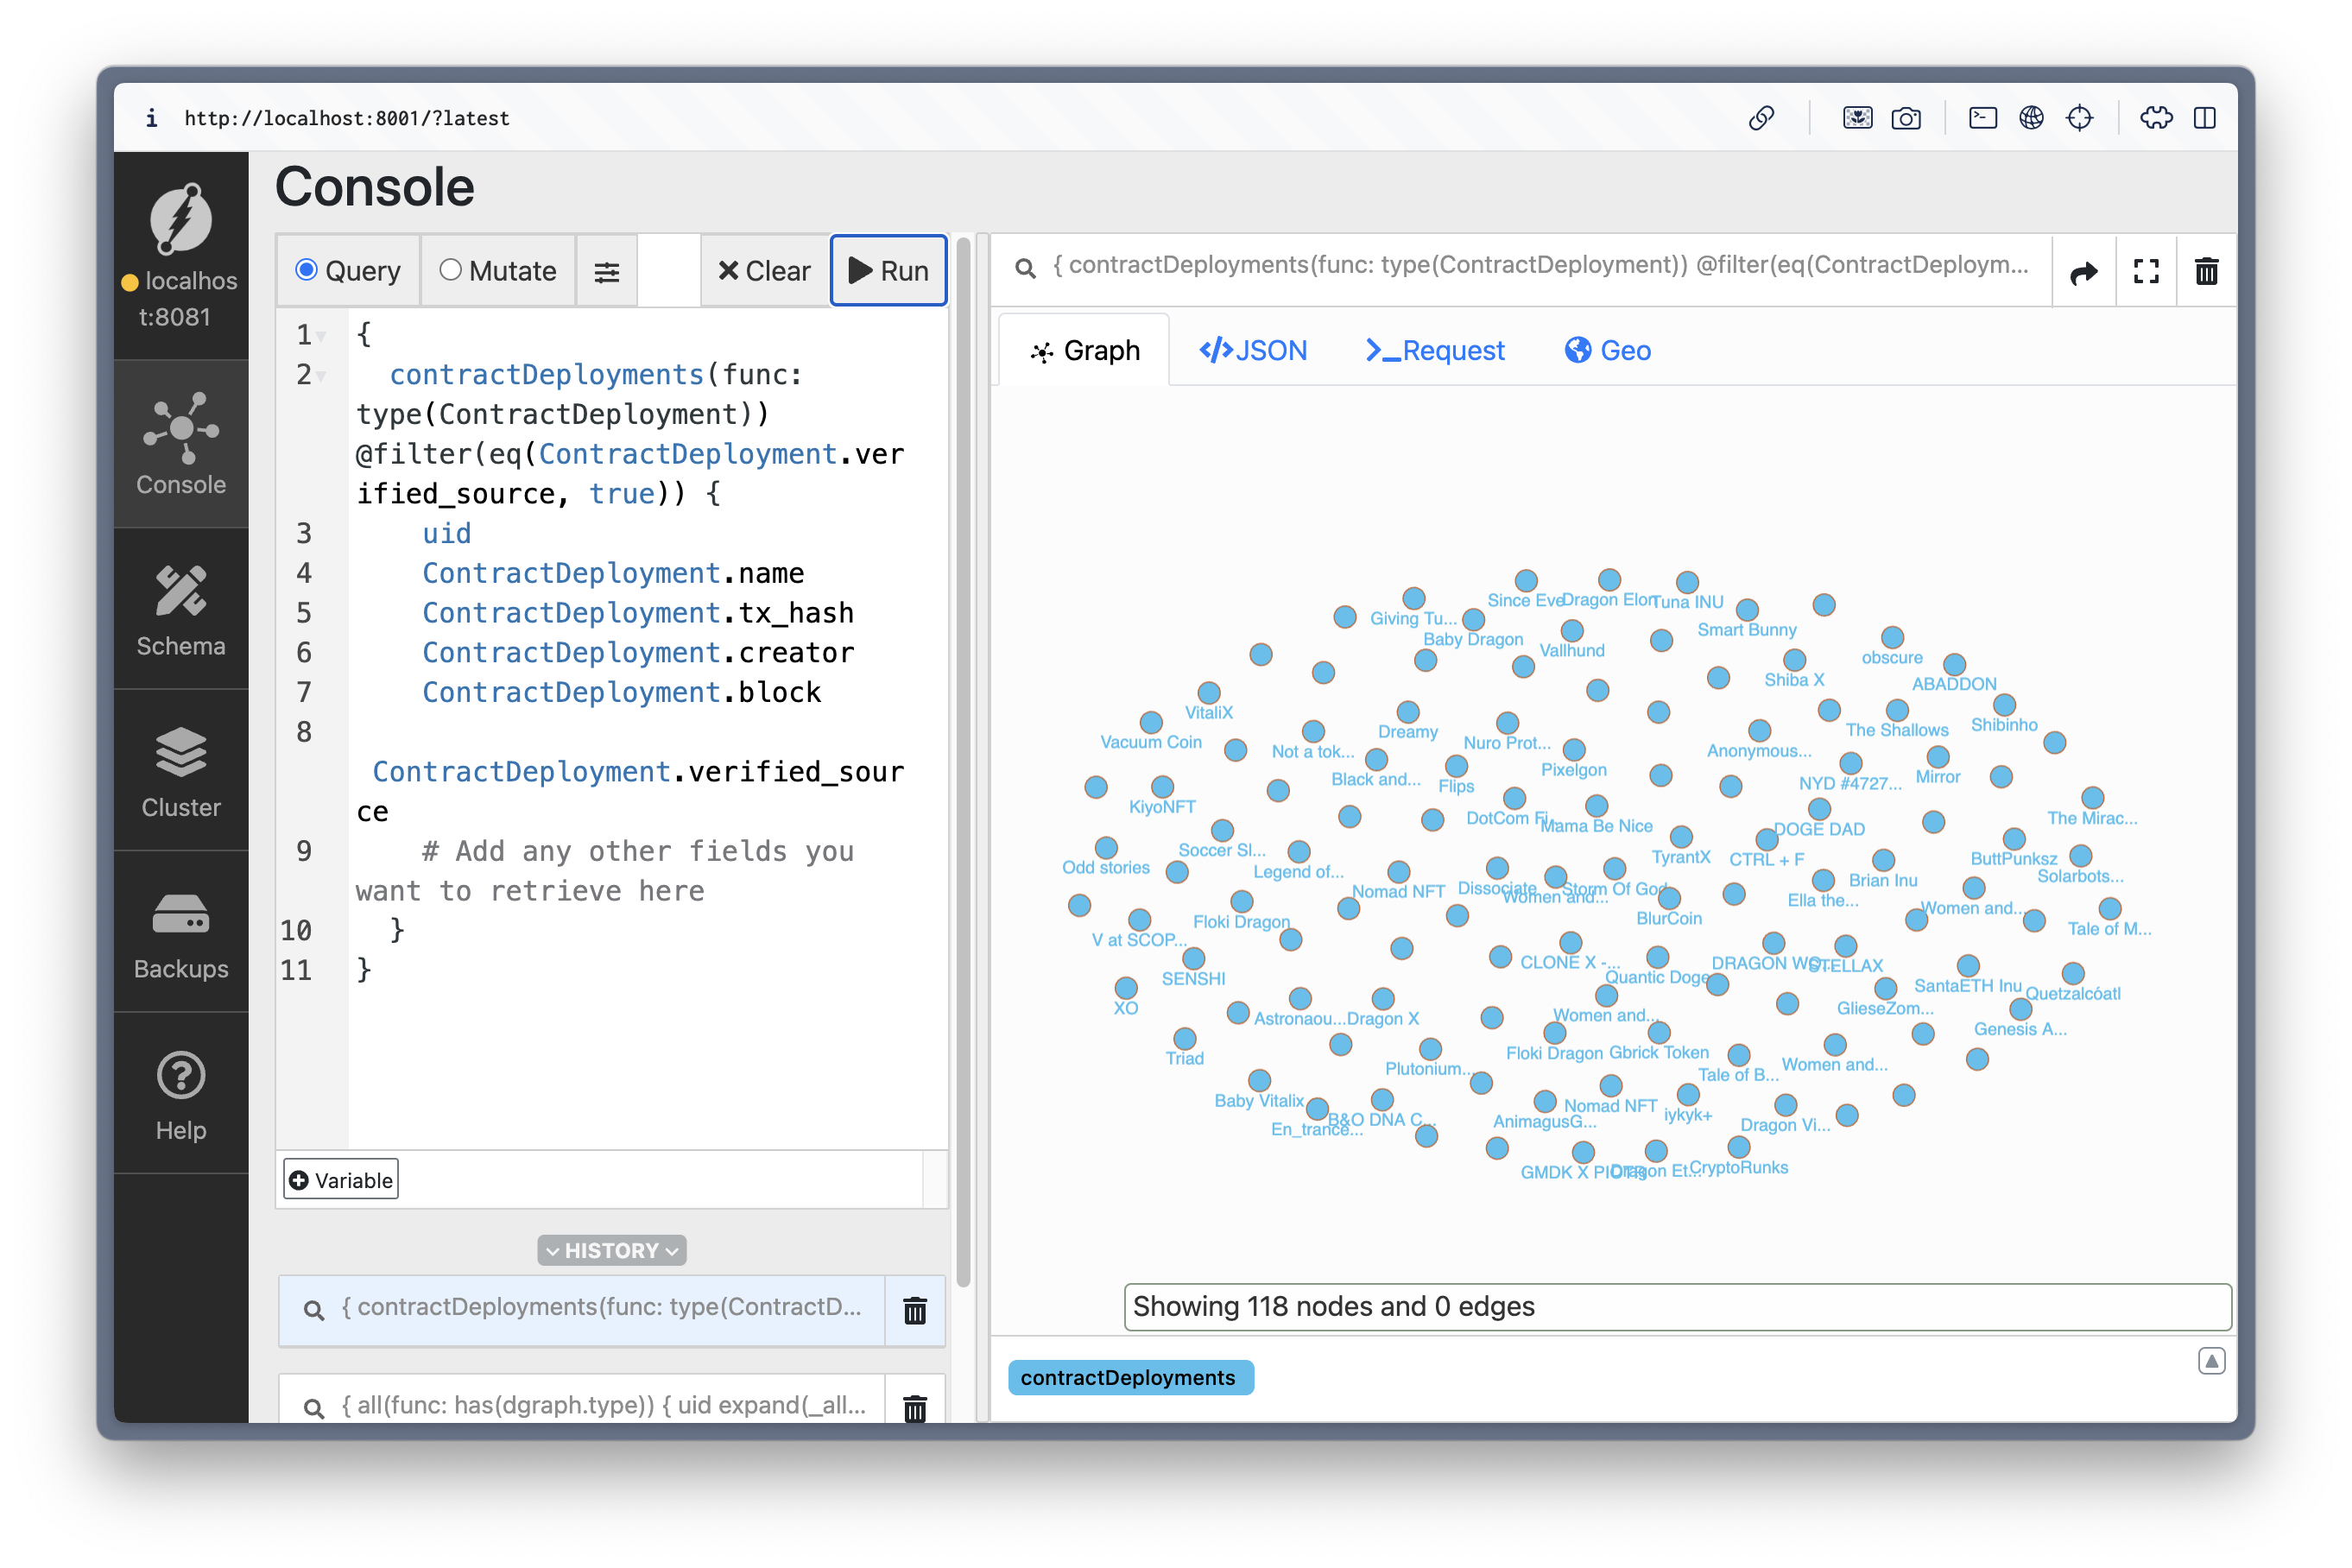
\includegraphics[width=1\textwidth]{resources/appendix/hasil-data-1.png}
	\caption{Hasil ekstraksi data}
	\label{image:hasil-data-1}
\end{figure}

\begin{figure}[ht]
	\centering
	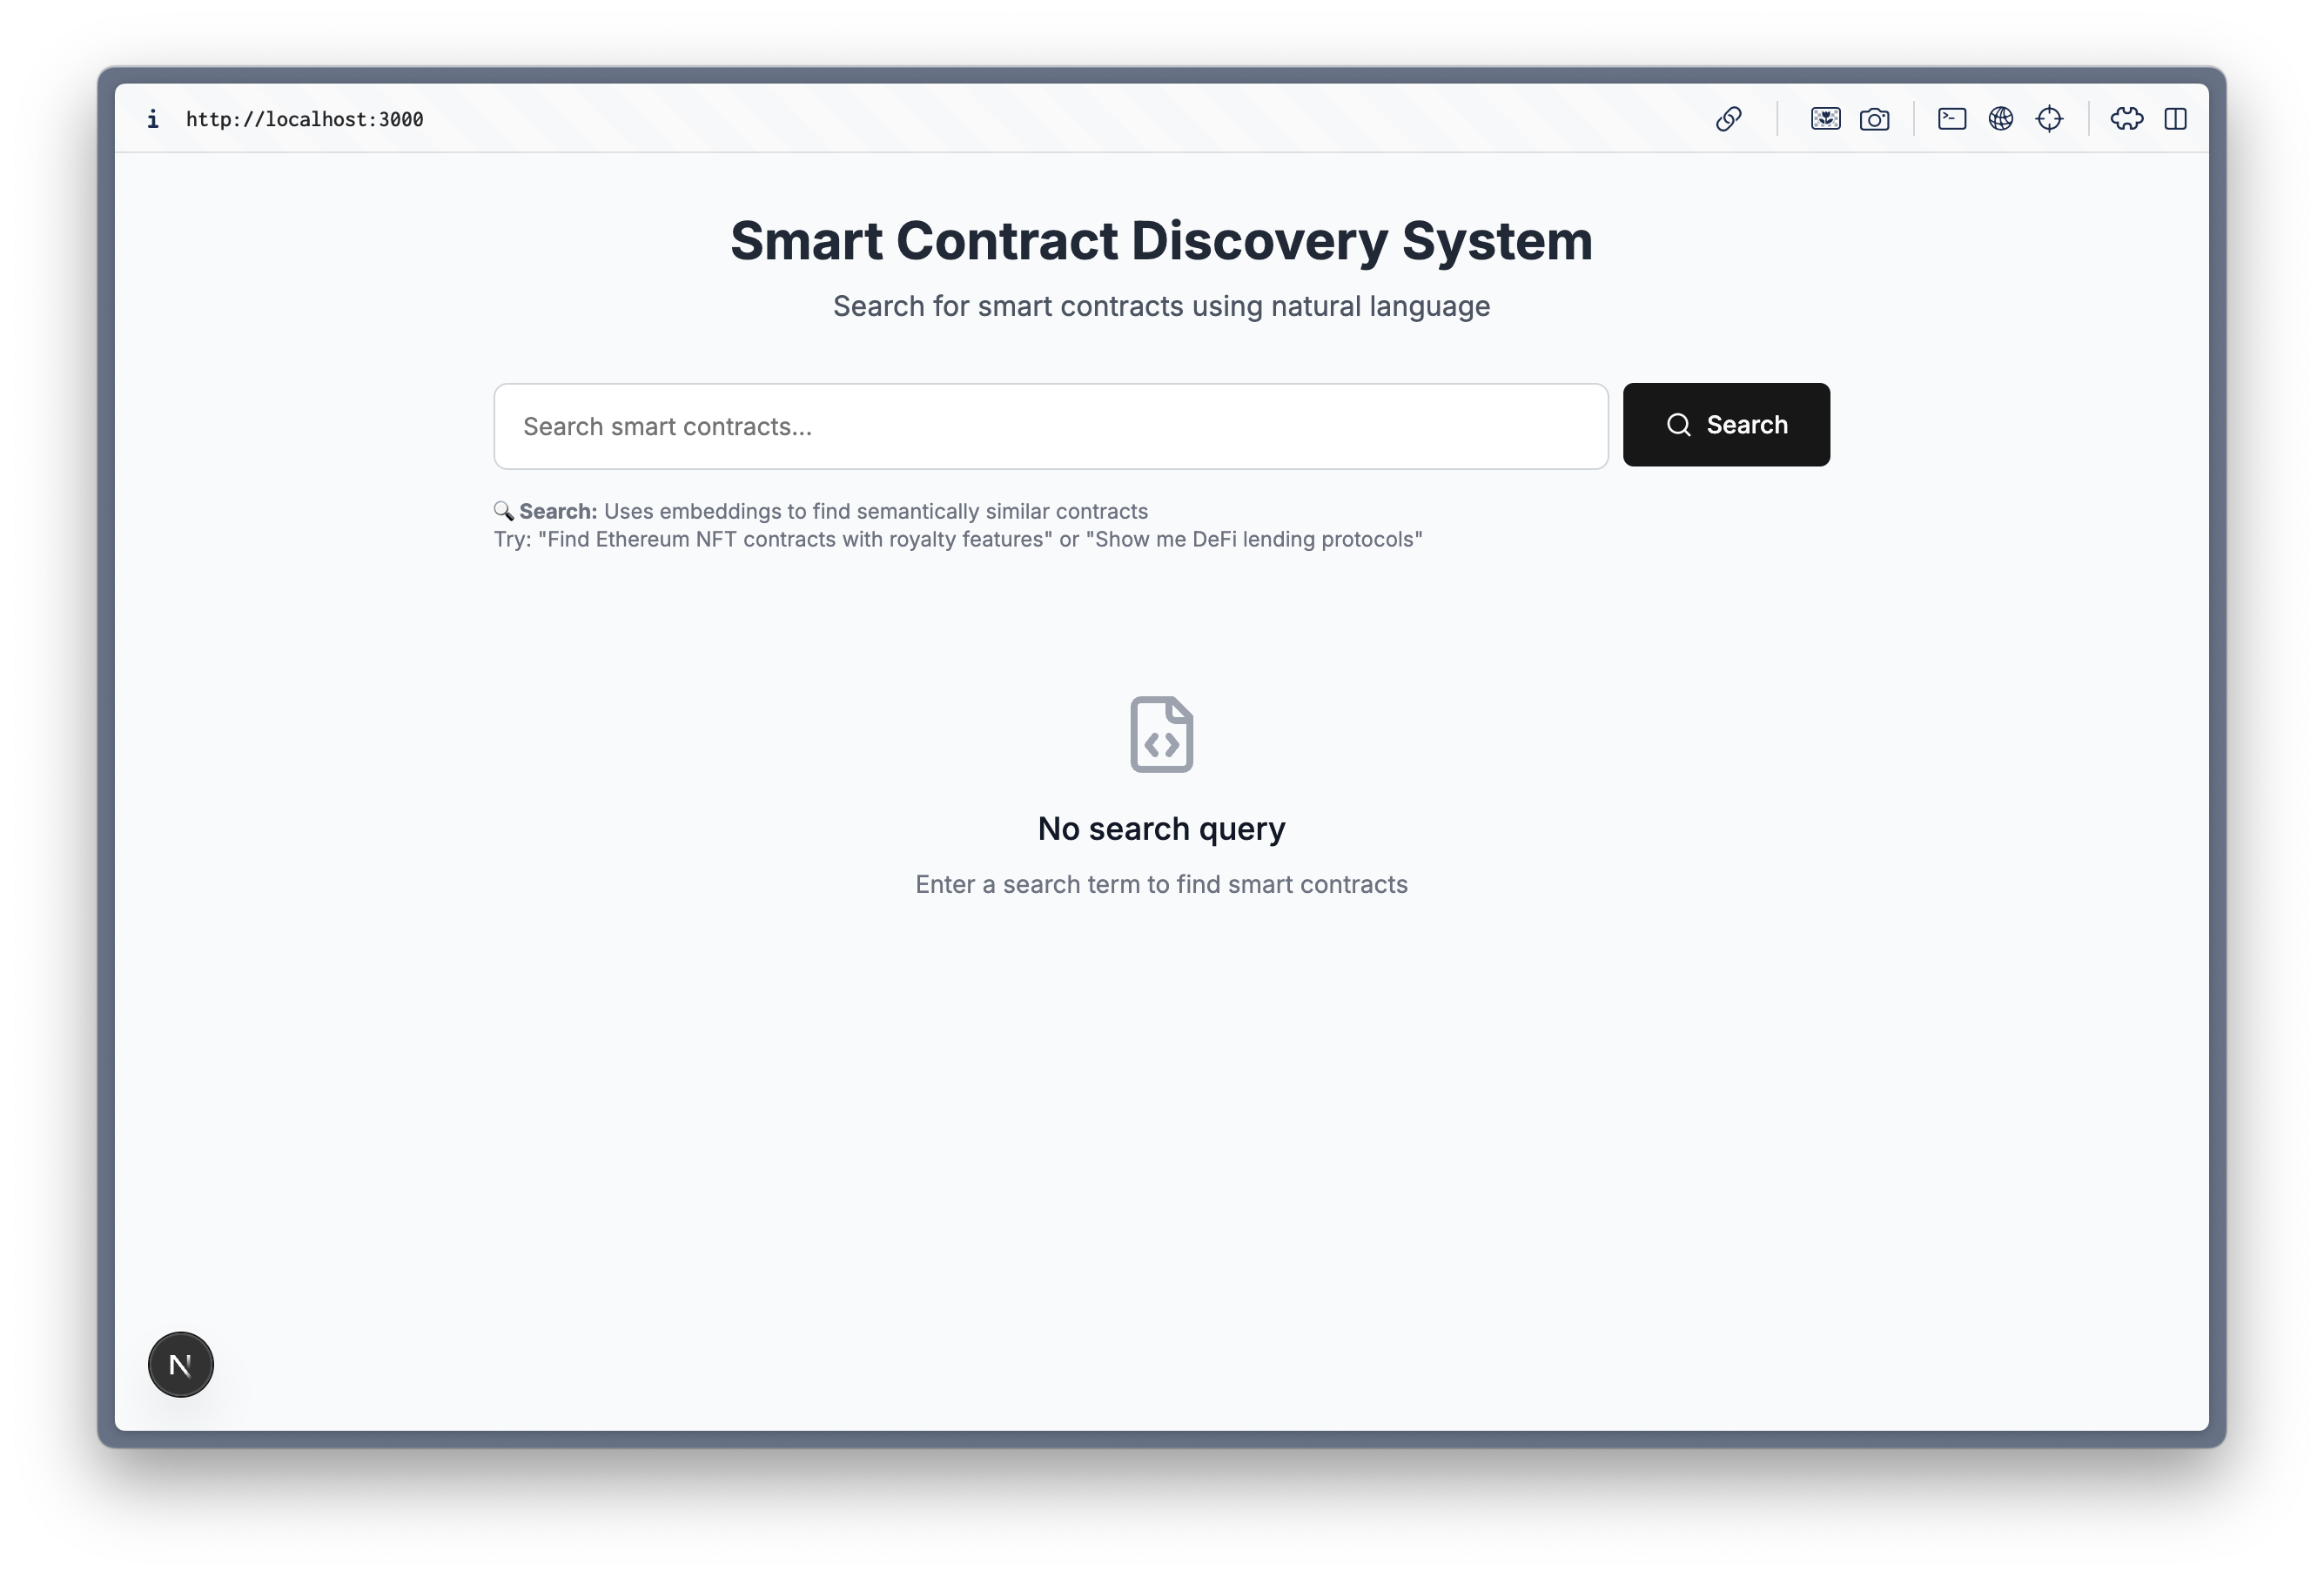
\includegraphics[width=1\textwidth]{resources/appendix/hasil-gui-1.png}
	\caption{Hasil antarmuka pengguna}
	\label{image:hasil-gui-1}
\end{figure}

\begin{figure}[ht]
	\centering
	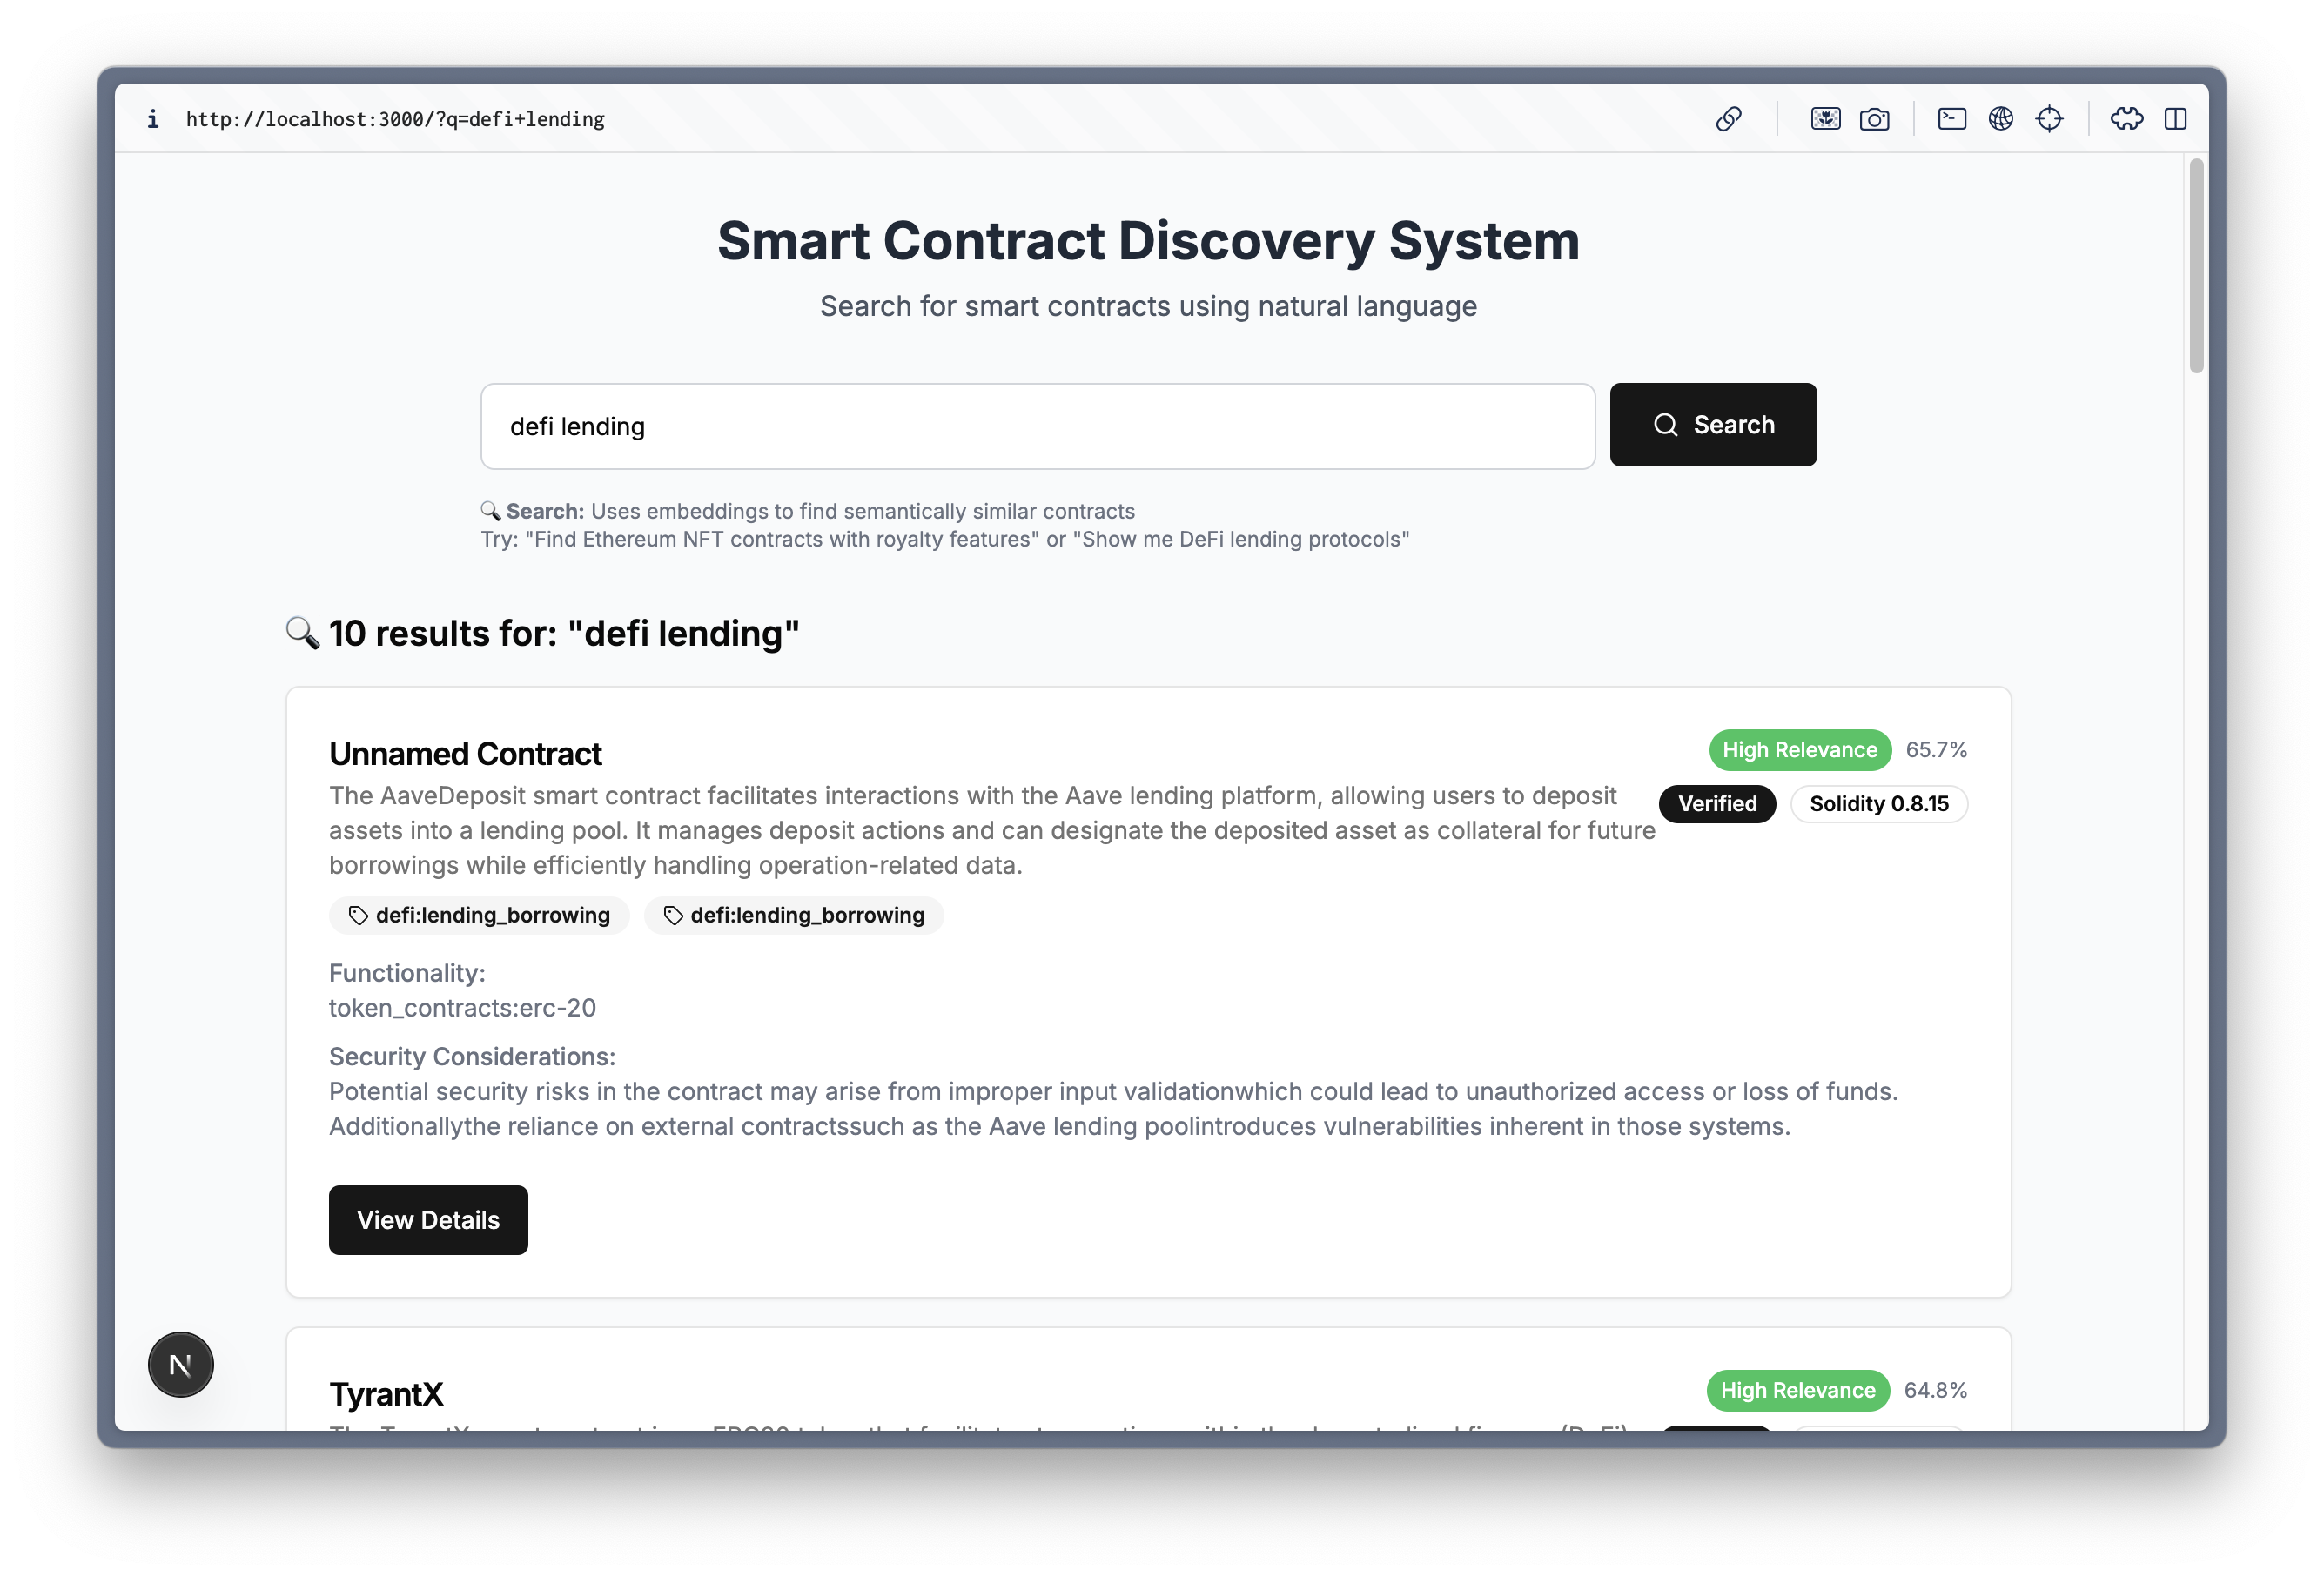
\includegraphics[width=1\textwidth]{resources/appendix/hasil-gui-2.png}
	\caption{Hasil antarmuka pengguna}
	\label{image:hasil-gui-2}
\end{figure}

\begin{figure}[ht]
	\centering
	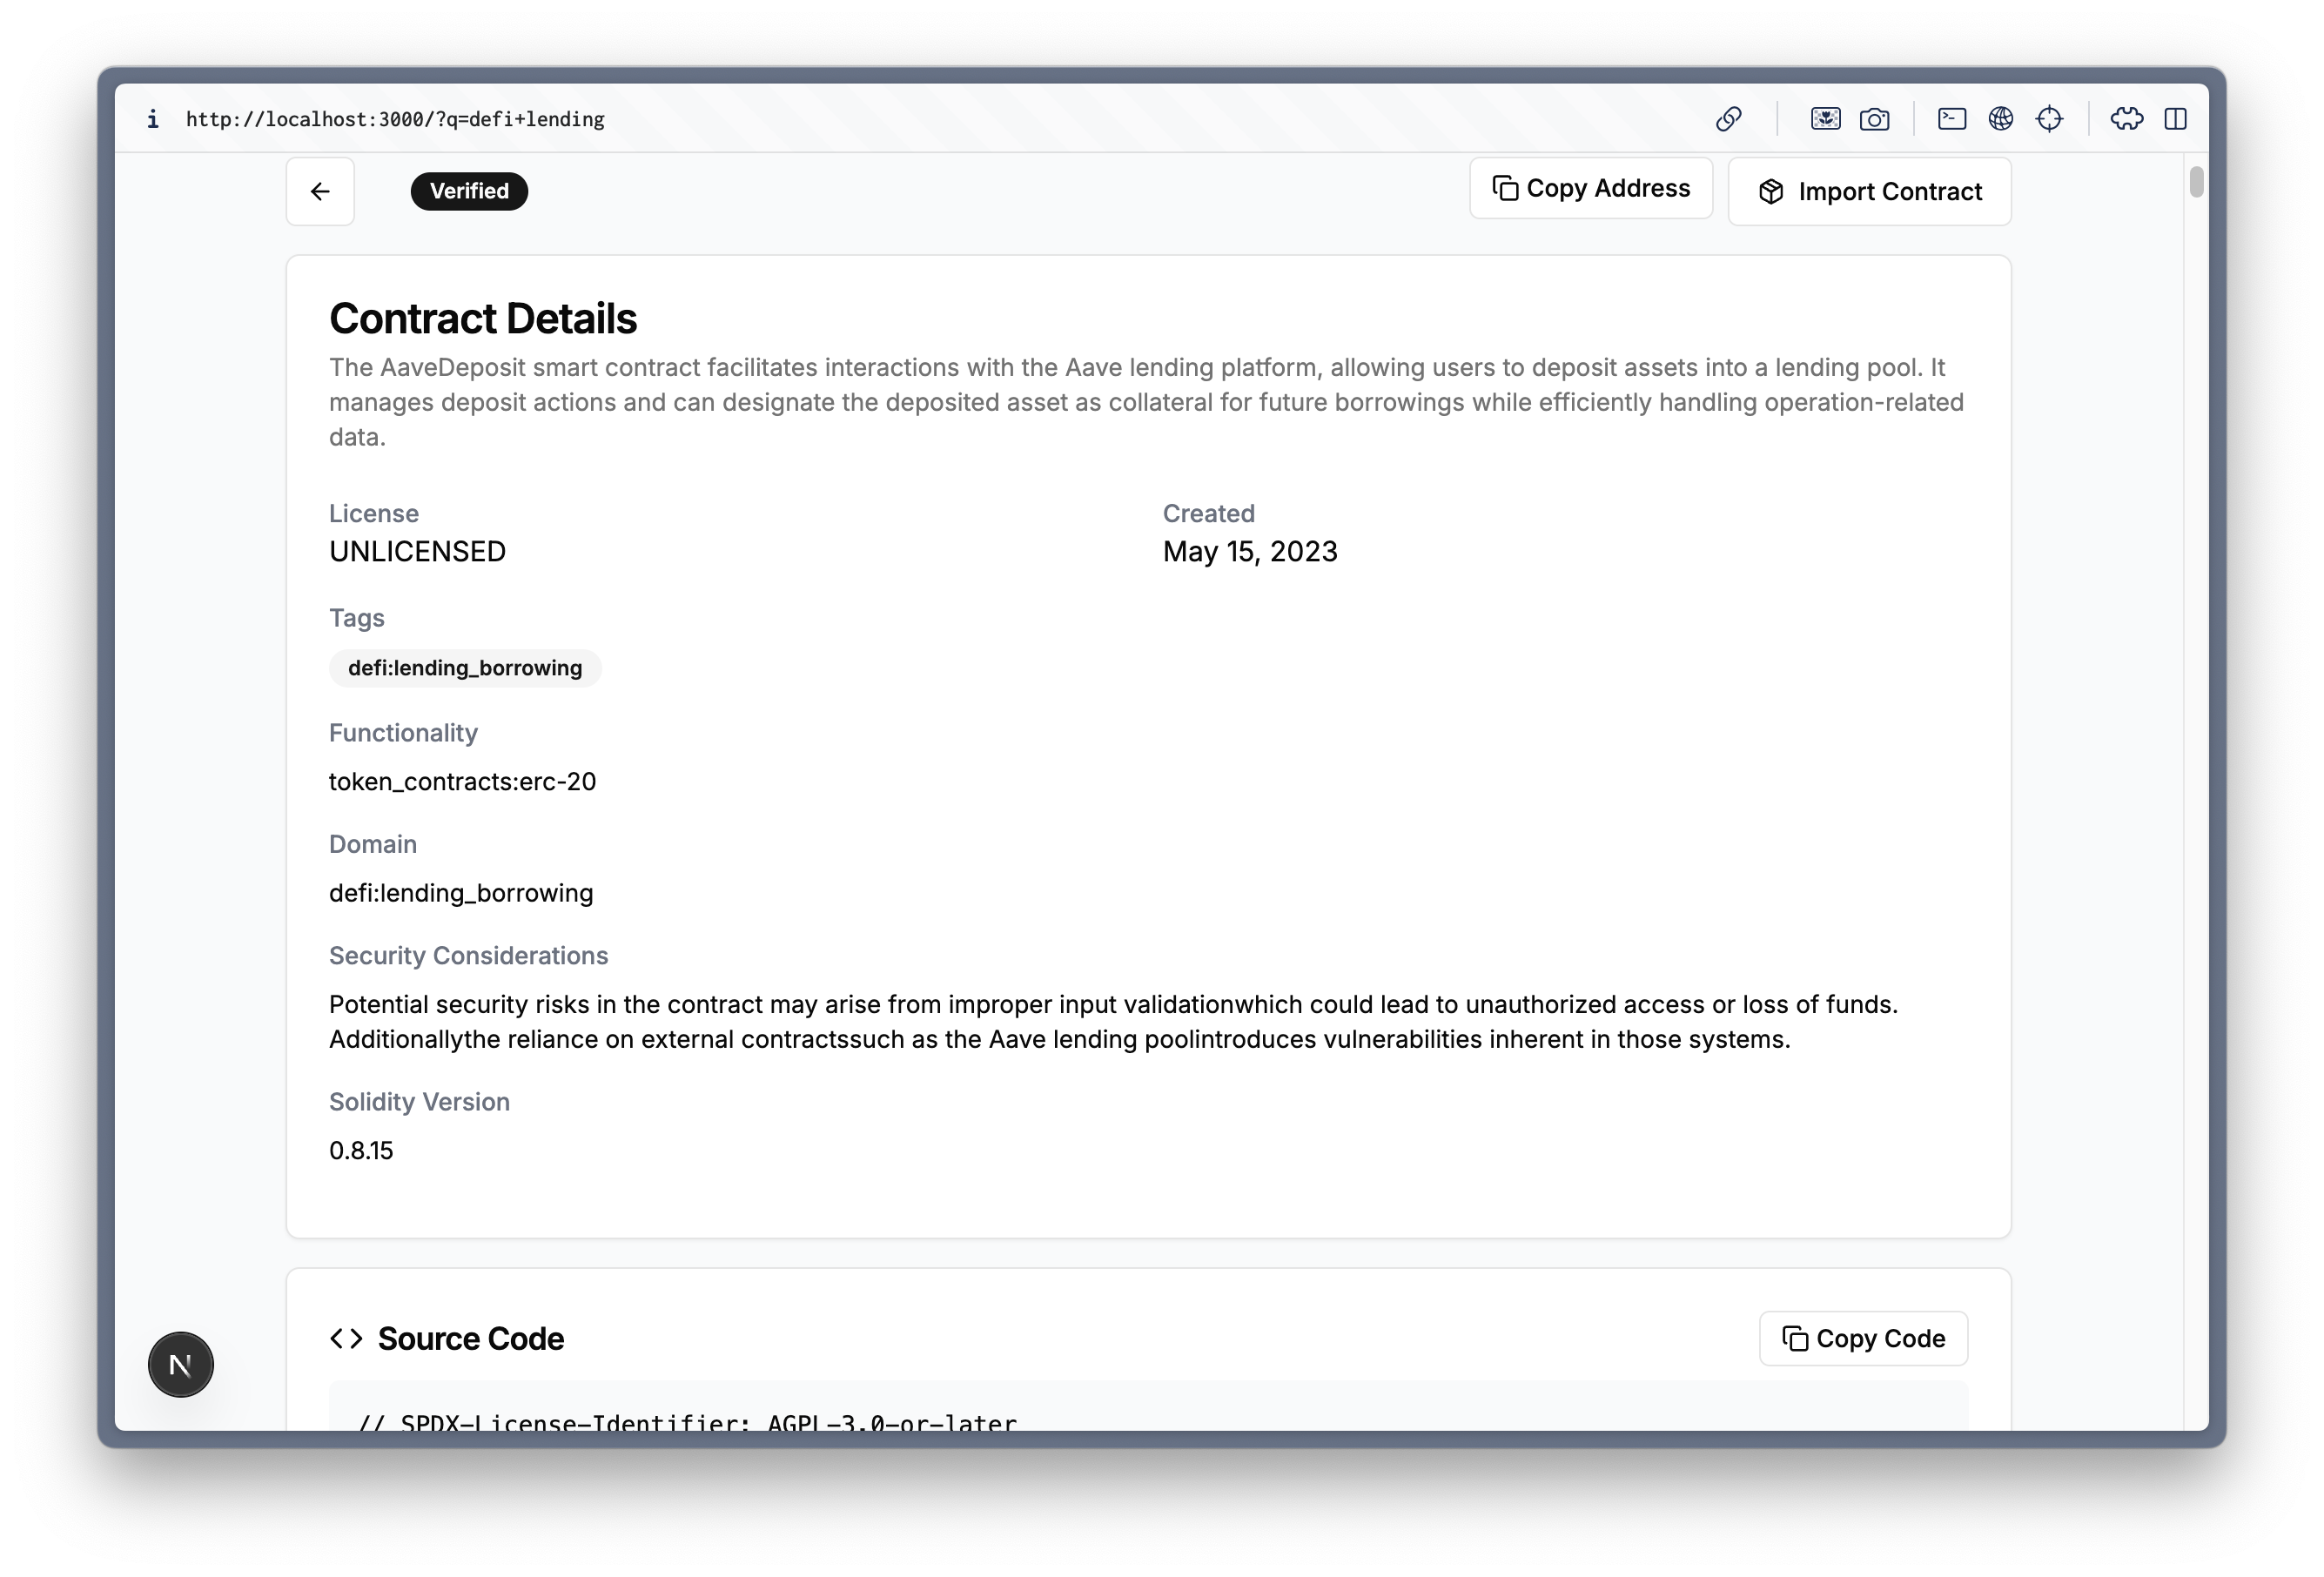
\includegraphics[width=1\textwidth]{resources/appendix/hasil-gui-3.png}
	\caption{Hasil antarmuka pengguna}
	\label{image:hasil-gui-3}
\end{figure}

\begin{figure}[ht]
	\centering
	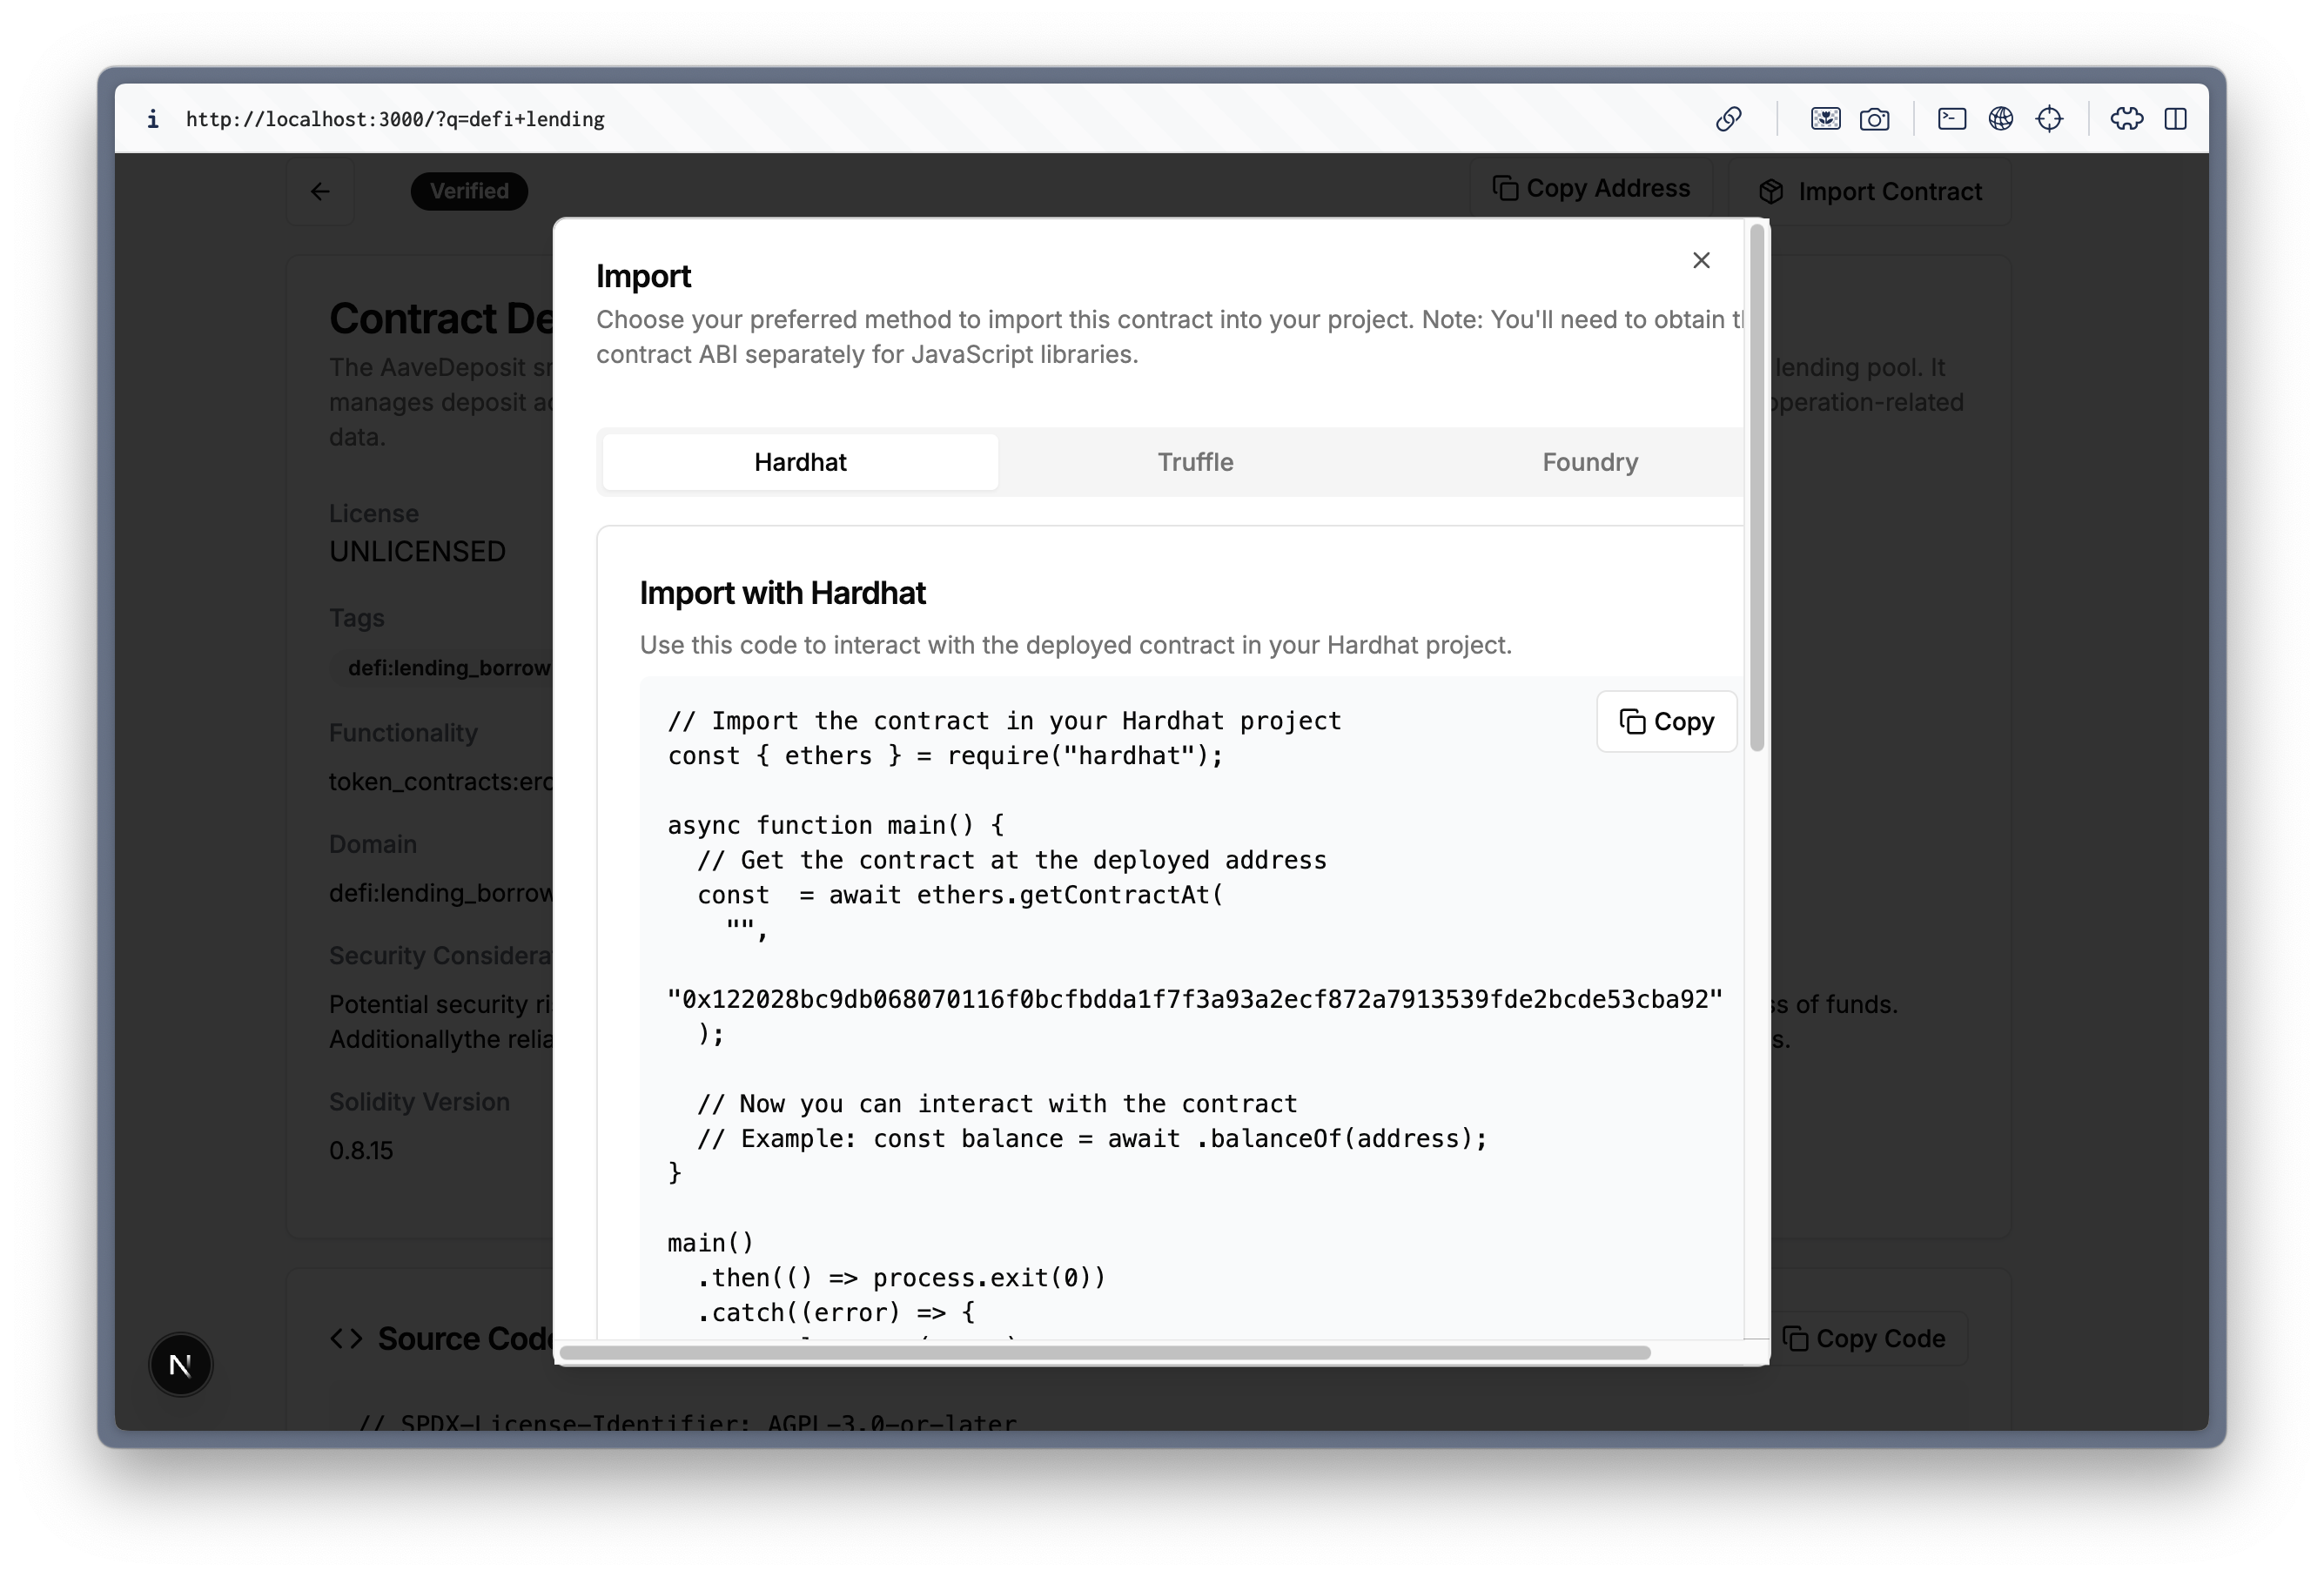
\includegraphics[width=1\textwidth]{resources/appendix/hasil-gui-4.png}
	\caption{Hasil antarmuka pengguna}
	\label{image:hasil-gui-4}
\end{figure}

\begin{figure}[ht]
	\centering
	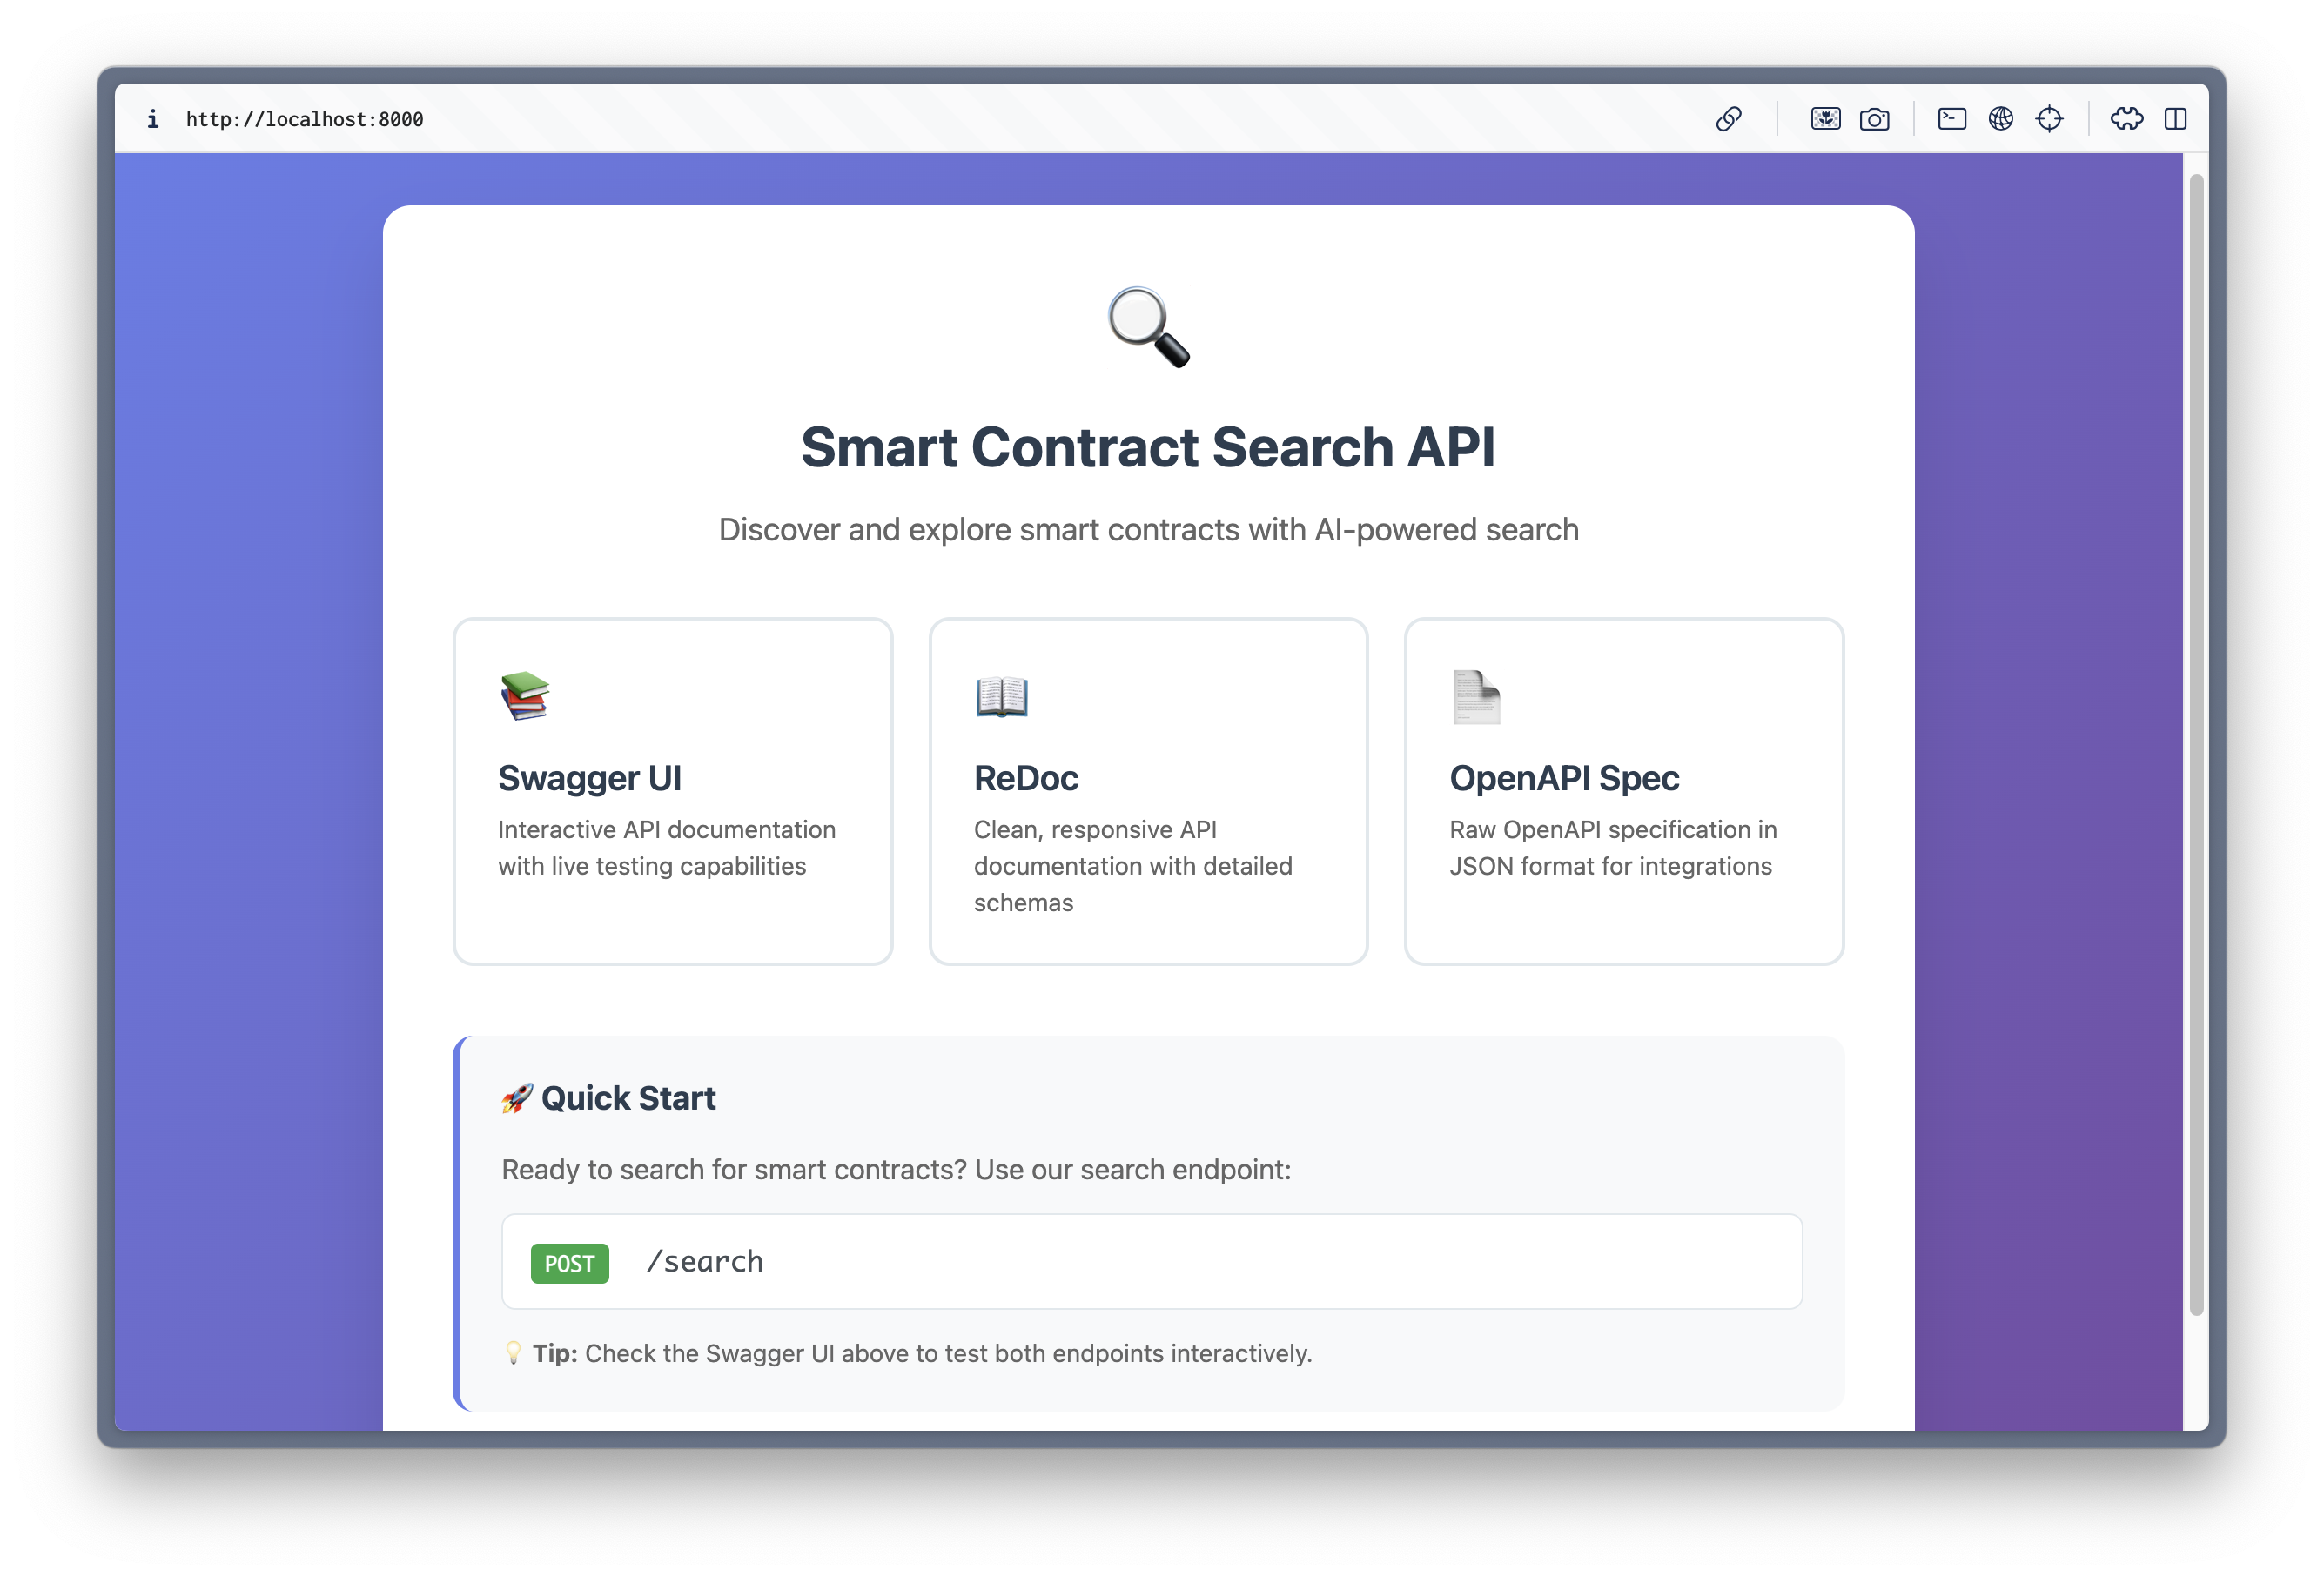
\includegraphics[width=1\textwidth]{resources/appendix/hasil-api-1.png}
	\caption{Hasil antarmuka pengguna}
	\label{image:hasil-api-1}
\end{figure}

\begin{figure}[ht]
	\centering
	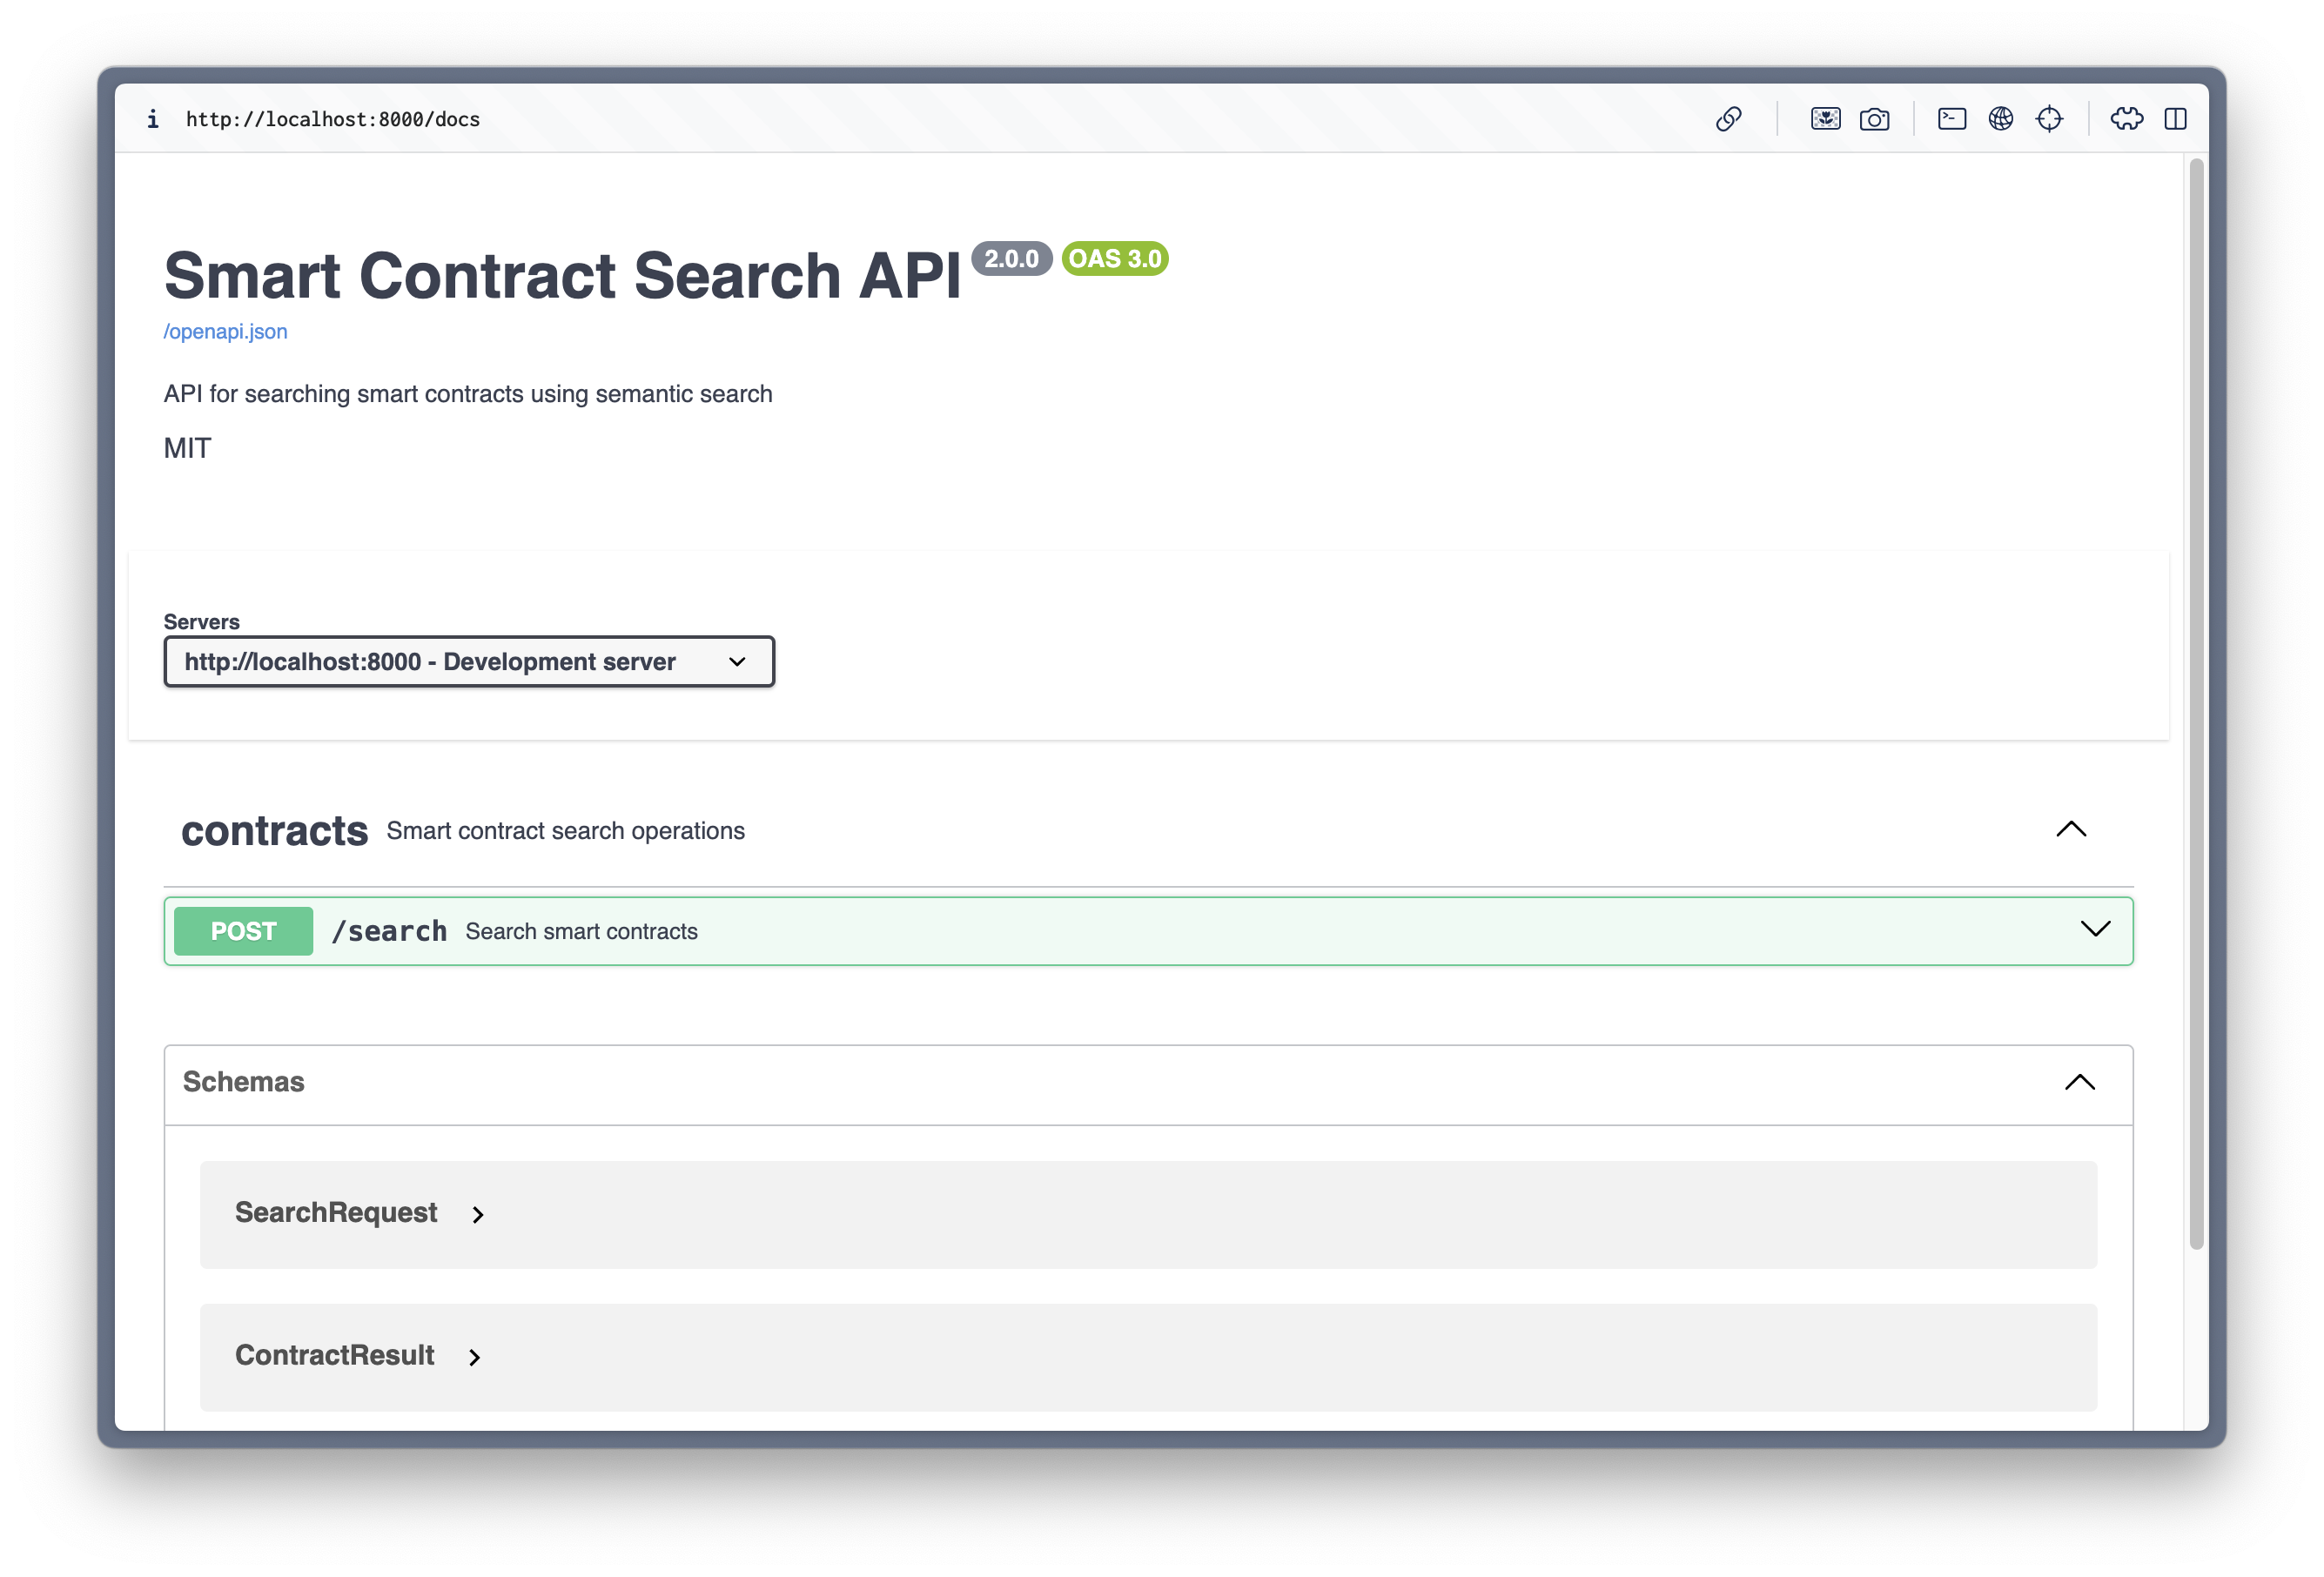
\includegraphics[width=1\textwidth]{resources/appendix/hasil-api-2.png}
	\caption{Hasil antarmuka pengguna}
	\label{image:hasil-api-2}
\end{figure}

\begin{figure}[ht]
	\centering
	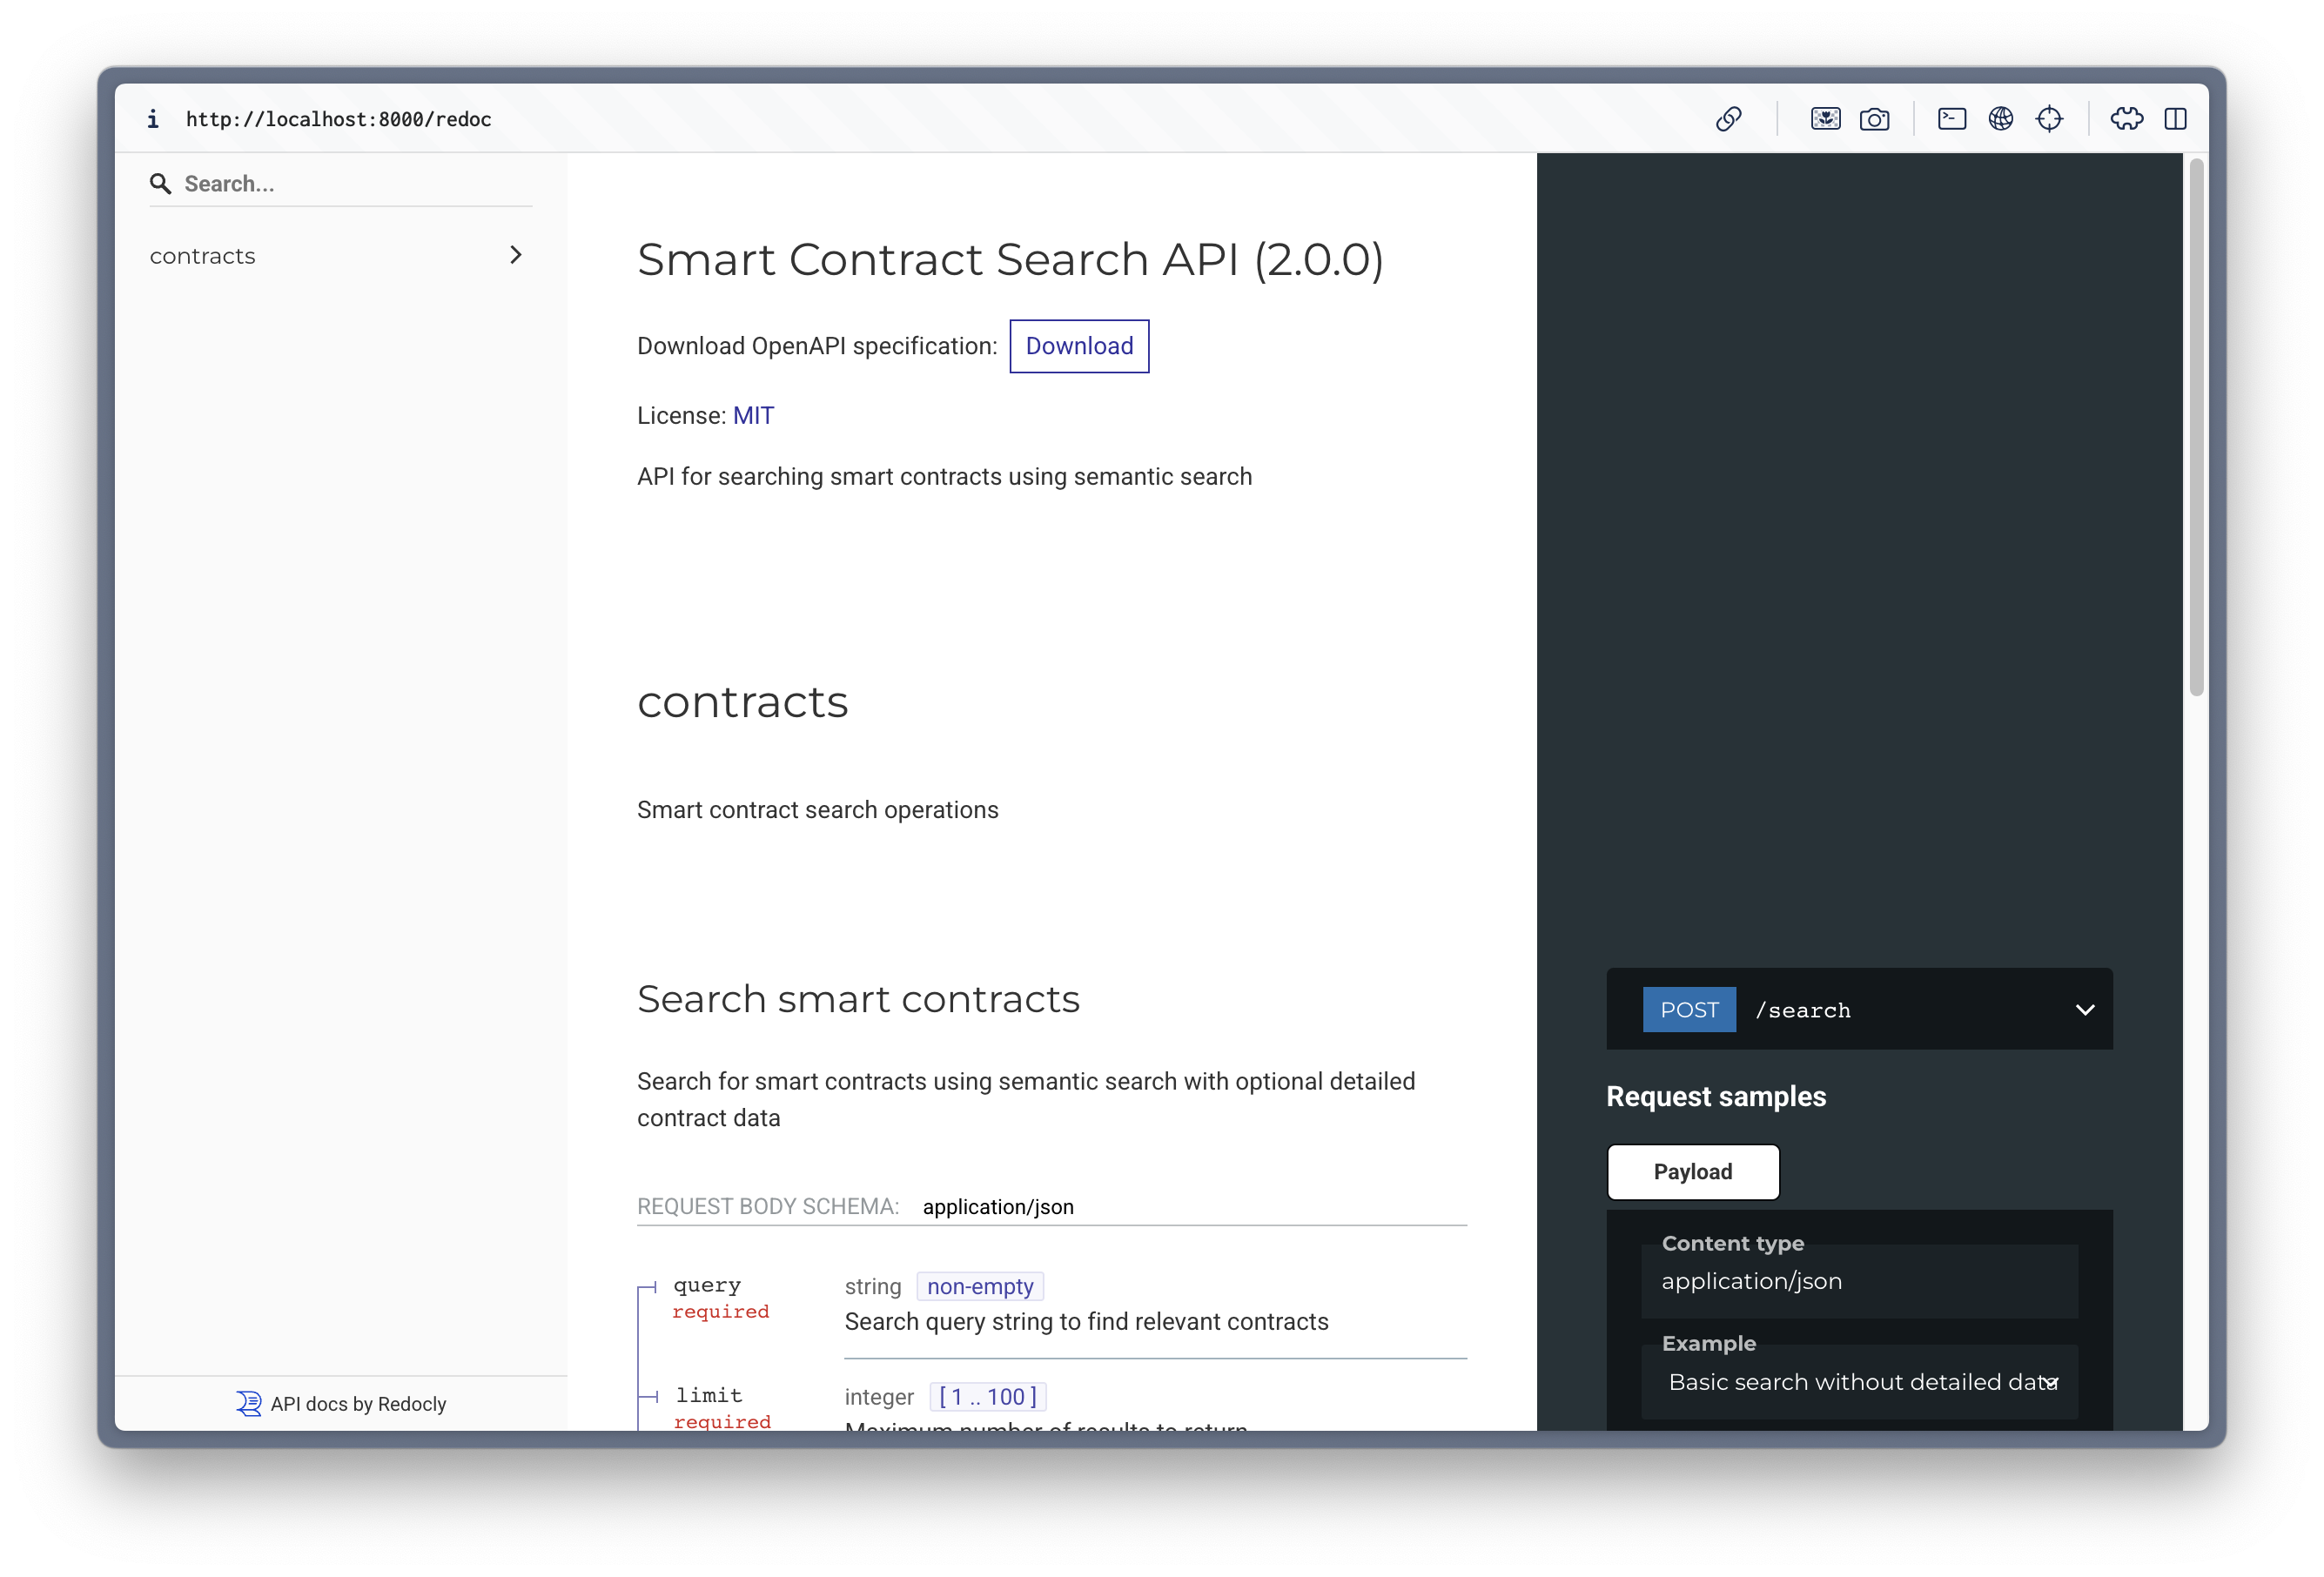
\includegraphics[width=1\textwidth]{resources/appendix/hasil-api-3.png}
	\caption{Hasil antarmuka pengguna}
	\label{image:hasil-api-3}
\end{figure}


\end{document}
